%scrartcl: Für kürzere Ausarbeitungen. Beginnt mit section, es gibt keine chapter
%scrreprt: Für längere Ausarbeitungen (Bacherlo oder Master Thesis). Beginnt chapter
\documentclass[pdftex,a4paper,abstracton,11pt,parskip=half,bibtotocnumbered]{scrartcl} 

% Je nach LaTeX Compiler werden etwas andere Bibliotheken verwendet.
% Das Paket iftex erlaubt es, den Compiler zu überprüfen
\usepackage{iftex}

\usepackage[ngerman]{babel} % Einstellungen für den deutschen Sprachraum, neue deutsche Rechtschreibung
\ifPDFTeX
  \usepackage[utf8]{inputenc} % Umlaute erkennen. Als Option in "[] " die vom Editor verwendete Zeichencodierung auswählen
  \usepackage[T1]{fontenc}
\fi

% Für kompakter Aufzählungen
\usepackage{paralist}

\usepackage[style=ieee,backend=bibtex]{biblatex}
\addbibresource{literatur/literatur.bib}

% Für Abbildungen
\usepackage{graphicx}
\graphicspath{{./abbildungen/}}

% Ändert die Überschrift des Abstracts.
% Falls kein Abstract benötigt wird, kann die Option "abstracton" ganz oben in \documentclass entfallen.
\renewcommand{\abstractname}{Zusammenfassung}



\title{Neugestaltung von Schüler Online: Eine Beobachtungs- und Interviewstudie zur Identifikation von Problemstellen und Nutzerbedürfnissen, um die Effektivität sowie die Zufriedenstellung des Schulpersonals beim Erfüllen von Kernaufgaben der Webanwendung zu optimieren}
\author{Lukas Wessel}
\date{\today}



\begin{document}

\makeatletter
\begin{titlepage}
	\centering
	{\scshape\LARGE Fachhochschule Südwestfalen \par}
	\vspace{1cm}
%	{\scshape\Large Merkblatt\par}
	\vspace{1.5cm}
	{\huge\bfseries \@title\par}
	\vspace{3cm}
	{\Large \@author\par}
	\vspace{1cm}
	{\Large \@date\par}
	\vfill

	\raggedright
%	{\large Eingereicht bei:\par}
%	{\large Betreuer 1}
\end{titlepage}
\makeatother

\thispagestyle{empty}
\begin{abstract}
%Ein Abstrakt, also eine Kurzzusammenfassung der Arbeit ist bei einer schriftlichen Ausarbeitung nicht unbedingt notwendig.
%Bei umfangreicheren Arbeiten, also z.~B. einer Bachelor- oder Master-Thesis, sollte die Ausarbeitung in jedem Fall mit einem \textit{Abstract} beginnen.
Schriftliche Ausarbeitungen sind  wissenschaftliche Texte, die in ihrem formalen Aufbau bestimmten Richtlinien entsprechen müssen.
Dies gilt im Besonderen für Abschlussarbeiten (Bachelor- oder Masterarbeiten), aber prinzipiell auch für kürzere Aufsätze, Hausarbeiten und Projektberichte.
In diesem Leitfaden soll es darum gehen, wie Sie Ihre Ausarbeitung strukturell aufbauen sollten und welche Qualitätskriterien für die äußere und sprachliche Form gelten.
Bei einer typischen Projekt-, Bachelor- oder Masterarbeit macht die schriftliche Ausarbeitung nur einen Teil der Arbeitslast aus, ist aber gleichzeitig das wichtigste Kriterium für die Bewertung.
Daher ist es ratsam, sich möglichst frühzeitig mit den inhaltlichen und formalen Anforderungen wissenschaftlicher Texte vertraut zu machen und diese bei der Anfertigung eigener Ausarbeitungen zu berücksichtigen.
\end{abstract}

\vfill
\tableofcontents
\pagebreak

\setcounter{page}{1}
\title{Neugestaltung von Schüler Online: Eine Beobachtungs- und Interviewstudie zur Identifikation von Problemstellen und Nutzerbedürfnissen, um die Effektivität sowie die Zufriedenstellung des Schulpersonals beim Erfüllen von Kernaufgaben der Webanwendung zu optimieren}

\section{Einleitung}

Das zentrale Anliegen dieser Projektarbeit ist die Untersuchung der Webanwendung "Schüler Online 2.0". Um ein tieferes Verständnis für ihre Funktionalität in der Praxis zu erlangen, werden fünf Sekretärinnen an fünf verschiedenen Schulen mittels eines semistrukturierten Leitfadeninterviews befragt und offen beobachtet. Die Ergebnisse werden im Rahmen dieser Arbeit ausgewertet und analysiert.

Die Relevanz des Themas ergibt sich aus dem Bedarf des Entwicklungsteams, die Verwendungsweise der Anwendung in der Praxis zu verstehen. Trotz vorhandener Forschungen und Literatur über generelle Probleme im Hinblick auf Effektivität und Zufriedenheit sowie über diverse Heuristiken, fehlen spezifische Erkenntnisse für die untersuchte Webanwendung. Die Erforschung dieser Aspekte zielt darauf ab, das System zu optimieren, sodass Schulpersonal Bewerbungen von Schülern effektiv und zufriedenstellend bearbeiten kann. Aspekte der Effizienz sind nicht Gegenstand dieser Studie.

Das Forschungsziel ist es, Einblicke in die Problemstellen zu gewinnen, die das Schulpersonal während des Bewerbungsprozesses eines Schülers hindern könnten, seine Ziele effektiv zu erreichen. Dabei soll untersucht werden, ob die Testpersonen die an sie gestellten Aufgaben mit der Anwendung "Schüler Online 2.0" erfolgreich bewältigen können. 

Die Forschungsmethode umfasst qualitative Auswertungen der Interviews und Beobachtungen, wobei die Testpersonen drei konkrete Aufgaben innerhalb der Anwendung bewältigen sollen. Die Arbeit wird überwiegend induktiv betrieben und versucht, spezifische Erkenntnisse für das untersuchte System zu generieren, um es letztendlich zu verbessern.

Es sei jedoch darauf hingewiesen, dass diese Studie keine konkreten Maßnahmen oder Handlungsanweisungen behandelt. Vielmehr konzentriert sie sich auf die Identifizierung möglicher Problemstellen und Nutzerbedürfnisse, um einen fundierten Ausgangspunkt für zukünftige Forschungen und Entwicklungen zu bieten.

Im Rahmen dieser Studie sollen die folgenden Leitfragen beantwortete werden: 
\begin{itemize}
    \item Wovon handelt Schüler Online, welche Kernaufgaben bildet es ab und welche werden in dieser Studie analysiert? (LF1)% (Theorie)
    \item Wie kann Effektivität im Kontext der Untersuchung definiert werden? (LF2)% (Theorie)
    \item Wie kann Zufriedenheit im Kontext der Untersuchung definiert werden? (LF3)% (Theorie)
    \item Welche typische Problemstellen und Nutzerbedürfnisse gibt es bei Webanwendungen? (LF4)% (Theorie)
    \item Wie sollte so ein Fragebogen aussehen? (LF5)% (Ergebnisteil)
    % \item Welcher Nutzerbedürfnisse gibt es und inwieweit werden sie von der Anwendung erfüllt? (LF7)% (Ergebnisteil)
    \item Welche Problemstellen gibt es bei in Anwendung? (LF6)% (Ergebnisteil)
    \item Erreichen die Nutzer effektiv und zufriedenstellend ihre Ziele? (LF7)% (Diskussion)
\end{itemize}

ALTERNATIV  

Im Rahmen dieser Studie werden mehrere zentrale Fragen untersucht: Zunächst wird die Webanwendung \glqq Schüler Online\glqq  beleuchtet, um zu klären, wovon sie handelt, welche Kernaufgaben sie abbildet, und welche speziell in dieser Studie analysiert werden (LF1). Anschließend wird die Effektivität im Kontext der Untersuchung definiert(LF2), sowie die Zufriedenheit im Kontext der Untersuchung festgelegt(LF3). Die Forschung zitiert typische Problemstellen und Nutzerbedürfnisse bei Webanwendungen(LF4). Zudem wird erörtert, wie ein entsprechender Fragebogen aussehen sollte, um die benötigten Daten zu sammeln (LF5). Weiterhin wird untersucht, welche Problemstellen bei der Anwendung konkret aufgetreten sind (LF6), und abschließend bewertet, ob die Nutzer effektiv und zufriedenstellend ihre Ziele erreichen (LF7).

\pagebreak
%Das Thema dieser Projektarbeit behandelt die Webanwendung textit{Schüler Online 2.0}. Hierzu %werden bei insgesamt fünf Sekretärinnen an fünf verschiedenen Schulen ein semistrukturiertes %Leitfadeninterview durchgeführt und die Testpersonen offen beobachtet, und im Rahmen dieser %Projektarbeit ausgewertet.
%
%Das Thema ist relevant, da dem Entwicklungsteam bislang keine Klarheit darüber vorliegt, wie %die Anwendung in der Praxis performt.
%Die Forschung wird überwiegend induktiv betrieben, es gibt zwar in der Literatur bereits %Erkenntnisse darüber, welche Probleme hinsichtlich Effektivät und Zufriedenstellung sowie %diverse Heuristiken, nicht allerdings speziell für die zu untersuchende Webanwendung. Ebendas %soll untersucht werden, damit die Anwender die Bewerbungen von Schülern effektiv und %zufriedenstellend erfassen und bearbeiten können.
%
%Das Ziel der Forschung ist es, einen Einblick zu gewinnen, welche Problemstellen und %Nutzerbedürfnisse das Schulpersonal beim Bewerbungsprozess eines Schülers und den Nutzer daran %hindern, sein Ziel effektiv und zufriedenstellend zu erreichen. Es soll herausgefunden werden, %ob die Testpersonen die Aufgabenstellungen effektiv und zufriedenstellend erledigen können. Die %Ergebnisse der Interviews und Beobachtungen werden hierfür qualitativ ausgewertet. Die %Forschung wird betrieben, indem Personen aus der genannten Gruppe drei Aufgaben in der %Anwendung Schüler Online bewältigen sollen. 




%Zu Beginn der Ausarbeitung ist es besonders wichtig, dem Leser zu erklären, warum Sie das Thema bearbeiten.
%Dabei ist nicht unbedingt Ihre eigene Motivation gemeint, sondern vielmehr die Frage, warum die Problemstellung Ihrer Arbeit relevant ist.
%Angemessene Motivationsgründe sind etwa:
%\begin{compactitem}
%\item Sie lösen ein Problem, für das es bisher keine, oder keine gute Lösung gibt.
%\item Ein Unternehmen kann Ihre Lösung einsetzen, um damit Profit zu erwirtschaften.
%\item Sie vergleichen verschiedene Produkte oder Methoden, um damit die Entscheidungsfindung bei der Auswahl zu erleichtern.
%\item Sie stellen ein komplexes Thema für eine bestimmte Zielgruppe angemessen dar.
%\end{compactitem}
Die zugrunde liegende Problemstellung ist relevant für den Hersteller der Anwendung \glqq Schüler Online"(\glqq Kommunales Rechenzentrum Minden/Ravensberg-Lippe"), da Unklarheit herrscht, ob die Anwender die Software korrekt bedienen können. Die Korrektheit ist auch für die Anwender wichtig, da die Anwendung das Schulgesetz abbilden soll und eine korrekten Erfüllung ermöglichen soll. Der Nutzer der Anwendung soll zufrieden sein, seine Erwartungen und Bedürfnisse an die Software sollen erfüllt werden. Mit der vorliegenden Studie soll geprüft werden, inwieweit die Software ebenjenen entspricht oder abweicht.

Es gibt zwar bereits Forschungen hinsichtlich häufig vorkommenden Problemstellen und Nutzerbedürfnissen von diversen Autoren, 
%wie bspw. 
allerdings liegt noch keine Forschung zur Webanwendung \glqq Schüler Online" im Bereich des Usability Engineerings vor. 

\section{Theoretischer Hintergrund}
\subsection{Die Webanwendung \textit{Schüler Online}}
Schüler Online ist eine Webapplikation, die die Anmeldung von Schülern an Schulen erleichtert. Die primär involvierten Parteien umfassen Schüler, Eltern und Schulen. Die Schulen bearbeiten hauptsächlich die Anmeldungen und entscheiden über Aufnahmen. Kreise und Gemeinden sind ebenfalls beteiligt, sie lesen Statistiken und kontrollieren die Schulpflicht. Ausbildungsbetriebe und Administratoren spielen auch eine Rolle; die Betriebe agieren als Partner für Ausbildungen, und die Administratoren pflegen die Stammdaten. Anmeldungen können von Schülern, Eltern, Schulen, Gemeinden oder Betrieben erstellt und modifiziert werden. Diese Ausarbeitung konzentriert sich auf den Prozess, bei dem Schulen selbst die Anmeldungen anlegen und die eingegangenen Anmeldungen bearbeiten.\cite{ProductOwner2023}

\subsection{Definition von Effektivität im Rahmen dieser Ausarbeitung }
Die ISO 9241-110 definiert Effektivität wie folgt: \glqq Effektivität = Die Genauigkeit und Vollständigkeit mit der Benutzer ein bestimmtes Ziel erreichen.\grqq{}\cite{ISO-9241-110}
In Anlehnung an diese Definition kann festgelegt werden, dass Effektivität im Sinne dieser Ausarbeitung das Ausmaß der Genauigkeit und Vollständigkeit mit dem die Studienteilnehmer die drei an sie gestellten Aufgaben erreichen. 

Erfolgskriterien, die darauf hinweisen, dass eine Aufgabe erfolgreich abgeschlossen wurde, sind: 
\begin{itemize}
    \item Die Navigation zur Aufgabe wurde erfolgreich abgeschlossen (EK1)
    \item Die Pflichtangaben wurden vollständig erfasst (EK2)
    \item Der Aufnahmestatus ist entweder \textit{Aufgenommen}, \textit{Abgelehnt} oder \textit{Warteliste} (EK3)
    \item Die Anmeldung wurde erfolgreich gespeichert (EK4)
\end{itemize}

\subsection{Definition von Zufriedenstellung im Rahmen dieser Ausarbeitung}
Die ISO 9241-110 definiert Zufriedenstellung: \glqq Das Ausmaß der Übereinstimmung der physischen, kognitiven und emotionalen Reaktionen des Benutzers, die aus der Benutzung eines Systems, eines Produkts oder einer Dienstleistung resultieren, mit den Benutzererfordernissen und Benutzererwartungen.\grqq{}\cite{ISO-9241-110} Hieran anknüpfend kann man für die vorliegende Studie festlegen, dass Zufriedenstellung das Ausmaß der Übereinstimmung zwischen den aus der Benutzung von \textit{Schüler Online} entstandenen Reaktionen des Schulpersonals und den Benutzererfordernissen und Benutzererwartungen ist. 

\subsection{Definition von Problemstellen im Rahmen dieser Ausarbeitung}
Im Rahmen dieser Arbeit bezieht sich der Begriff \textit{Problemstelle} auf spezifische Elemente der \textit{Schüler Online}-Anwendung, die bei ihrer Nutzung durch das Schulpersonal zu Defiziten in Bezug auf Effektivität und Zufriedenheit führen.

\subsection{Definition von Nutzerbedürfnissen im Rahmen dieser Ausarbeitung}
Stangl beschreibt den Begriff \textit{Bedürfnis} als \glqq das Verlangen oder der Wunsch, einen empfundenen oder tatsächlichen Mangel Abhilfe zu schaffen.\grqq{}\cite{stangl-beduerfnis} Dies wirft die Frage auf, was ein Mangel im Kontext einer Anmeldung an einer Schule für den Anwender bedeutet. Wenn man herkömmliche Anmeldungen mittels eines Papierformulars betrachtet, kann man hier argumentieren, dass mehrere Aspekte mangelhaft sind. Beispielsweise gibt es keine Validierung der Daten hinsichtlich Korrektheit oder Plausibilität.  Datenvalidierung könnte allerdings durch eine gute Kommunikation mit der abgebenden Schule abgesichert werden. Das Einlesen der Daten ist möglicherweise problematisch, da handschriftliches Ausfüllen unleserlich geschrieben sein kann. Eine Übertragung in verwendete Schulsoftware, wie \textit{SchILD}\footnote{SchILD ist eine so genannte Schulverwaltungssoftware, mit denen die Sekretariate die Schülerdaten ihrer aktuell an der Schule studierenden Schüler administrieren.} kann nur durch unkomfortables Abtippen erreicht werden.
Eine auf diesen Argumenten basierende modellhafte Definition im Kontext dieser Arbeit kann also lauten: \glqq Nutzerbedürfnisse ist das Verlangen oder der Wunsch, die Datenerfassung der Anmeldung weder unsicher, inkorrekt, unplausibel noch unkomfortabel zu vollziehen\grqq{}.

%\begin{itemize}
%    \item \textbf{Schlechte Navigationsstrukturen:} Wenn Nutzer Schwierigkeiten haben, sich auf einer Website zurechtzufinden, können sie ihre Ziele nicht effektiv erreichen. Eine klare, konsistente und intuitive Navigationsstruktur ist entscheidend.
%    \item \textbf{Nicht erfüllte Erwartungen:} Wenn das Design oder die Funktionalität der Anwendung nicht den Erwartungen der Nutzer entspricht, können diese ihre Ziele nicht effektiv erreichen. Beispielsweise kann eine Schaltfläche, die aussieht, als würde sie eine bestimmte Aktion auslösen, tatsächlich eine ganz andere Aktion auslösen.
%    \item \textbf{Mangel an Feedback:} Nutzer müssen wissen, was passiert, wenn sie eine Aktion ausführen. Wenn eine Anwendung nicht angemessen auf Nutzereingaben reagiert, kann dies zu Frustration und Ineffektivität führen.
%    \item \textbf{Nicht zugängliches Design:} Webanwendungen sollten für alle Benutzer, einschließlich Menschen mit Behinderungen, nutzbar sein. Eine Anwendung, die nicht die Richtlinien für Barrierefreiheit erfüllt, kann für einige Nutzer ineffektiv sein.
%    \item \textbf{Schlechte Leistung:} Langsame Ladezeiten oder technische Probleme können die Effektivität stark beeinträchtigen, da sie Nutzer daran hindern, ihre Ziele in einer angemessenen Zeit zu erreichen.
%    \item \textbf{Komplizierte oder überladene Benutzeroberflächen:} Wenn eine Benutzeroberfläche zu viele Optionen, zu viel Text oder zu viele Bilder enthält, kann dies Benutzer verwirren und ihre Fähigkeit, ihre Ziele effektiv zu erreichen, beeinträchtigen.
%    \item \textbf{Mangel an Suchfunktion oder ineffektive Suchfunktionen:} Eine effektive Suche ist für viele Webanwendungen entscheidend. Wenn Nutzer nicht finden können, was sie suchen, können sie ihre Ziele nicht effektiv erreichen.
%
%    %Bedienfehler
%    %Entspricht Gewohnten Abläufen
%    %Nimmt Arbeit ab
%    %Schwierige Bedienung
%    %Suchen nach: \glqq Common usability problems in web applications\grqq{} 
%\end{itemize}

%evtl. wie sieht das schulgesetz aus oder der Prozess


\section{Material und Methode}
\subsection{Teilnehmerauswahl}

In der vorliegenden wissenschaftlichen Arbeit wurde auf zwei divergierende Pools zur Rekrutierung der Teilnehmer zurückgegriffen. Der erste Rekrutierungspool umfasste diejenigen Individuen oder vermittelnden Kontakte\footnote{Ein vermittelnder Kontakt ist ein Kontakt, der einen potenziellen Studienteilnehmer aus seinem persönlichen Umfeld kontaktiert hat und diesen gefragt hat, ob er an der Studie teilnehmen möchte}, die eine Schulung für \textit{Schüler Online} besucht hatten. In diesen Schulungen wurde am Ende eine Folie präsentiert, die diese Studie vorstellte und um die Beteiligung der Anwesenden bat. Aus diesem Pool wurde die Sekretärin des Berufskollegs akquiriert.

Ein alternativer Weg zur Gewinnung von Teilnehmern war die Kaltakquise. Aus diesem Pool kamen alle weiteren Teilnehmer. Dabei wurden Schulen in zwei umliegenden Kreisen telefonisch kontaktiert und um ihre Teilnahme an der Studie gebeten. Aus Gründen der Vertraulichkeit und der Einhaltung von Verschwiegenheitsvereinbarungen ist es an dieser Stelle nicht möglich, konkrete Angaben zur Region zu machen.

Die Auswahl der Teilnehmer erfolgte basierend auf einer Reihe von Kriterien. Wesentlich war, dass die Teilnehmer in ihrem beruflichen Alltag das zu untersuchende Produkt sinnvoll einsetzen konnten - dies war ein entscheidendes Inklusionskriterium. Besonders geeignet waren daher Sekretariatsmitarbeiter, Schulverwaltungsassistenten und potenziell auch Schulleitungen. Als weiteres Inklusionskriterium war es erforderlich, dass die Teilnehmer aktiv in den genannten Berufen tätig und nicht in den Ruhestand getreten waren.

Im Gegenzug dazu wurden Auszubildende und Referendare von der Studie ausgeschlossen, da sie nur begrenzte Erfahrungen mit dem Tätigkeitsfeld der Software hatten. Dies stellte ein explizites Exklusionskriterium dar. Darüber hinaus spielten Faktoren wie Alter, Geschlecht, Berufserfahrung, ethnischer Hintergrund und sozioökonomischer Status der Teilnehmer bei der Rekrutierung keine Rolle.

Die Teilnahme an der Studie erforderte nur die Verfügbarkeit und die Bereitschaft der Teilnehmer, sich freiwillig zu engagieren. Es wurde darauf geachtet, dass keine Teilnahmeverpflichtungen, beispielsweise durch Vorgesetzte wie der Schulleitung, entstanden.

\subsection{Umgebungsbedingungen der Beobachtungen und Interviews}

Die Beobachtungen und Interviews wurden im Rahmen eines Feldtests abgehalten und fanden während der regulären Arbeitszeit an den gewohnten Arbeitsplätzen der Studienteilnehmer statt, um realistische Szenarien zu erzeugen. 

Die Durchführung der Interviews wurde während der Sommerferien terminiert. Es war von Bedeutung, den tatsächlichen Arbeitskontext der Teilnehmer einzubeziehen, um ein möglichst repräsentatives Bild ihrer Erfahrungen und Herausforderungen im Umgang mit dem untersuchten Produkt zu gewinnen.

\subsection{Erstellung des Fragebogens}

Die Formulierung des Fragebogens erfolgte durch eine Expertengruppe, die aufgrund ihrer beruflichen Rolle und Erfahrung eine hohe fachliche Expertise in Bezug auf die Anforderungen der zu untersuchenden Software besaßen. Diese Gruppe setzte sich zusammen aus Individuen, die im beruflichen Kontext die Anforderungen an die Software definierten und dokumentierten. Innerhalb dieser Gruppe gab es keinen Usability Experten, ledigliche einen Studenten, der das Fach \glqq Usability Engineering\grqq{} in seinem Studium belegte.

Um die Qualität und Eignung des Fragebogens zu gewährleisten, wurde dieser nach der Erstellung von einem Experten für Usability Engineering überprüft und auf seine inhaltliche Eignung hin bewertet.

Die Formulierung der Fragen folgte bestimmten Richtlinien: Sie sollten klar und verständlich sein und offen formuliert werden, um eine breite Palette von Antworten zu ermöglichen. Es war hier wichtig, dass der verwendete Sprachschatz laut Kruse den Kenntnissen eines Mitarbeitenden im Schulsekretariat entspricht.\cite{Kruse_2015} Dies gewährleistete, dass alle Teilnehmer die Fragen ohne zusätzliche Erläuterungen verstehen und beantworten können.

\subsection{Entwicklung von Aufgaben und Szenarien}
\begin{figure}[H]
    \caption{Einordnung der Aufgaben in den Gesamtkontext der Anwendung im Rahmen einer Beobachtungs- und Interviewstudie zur Bestimmung der Effektivität und Zufriedenstellung}
    \label{fig:EinordnungAufgaben}
    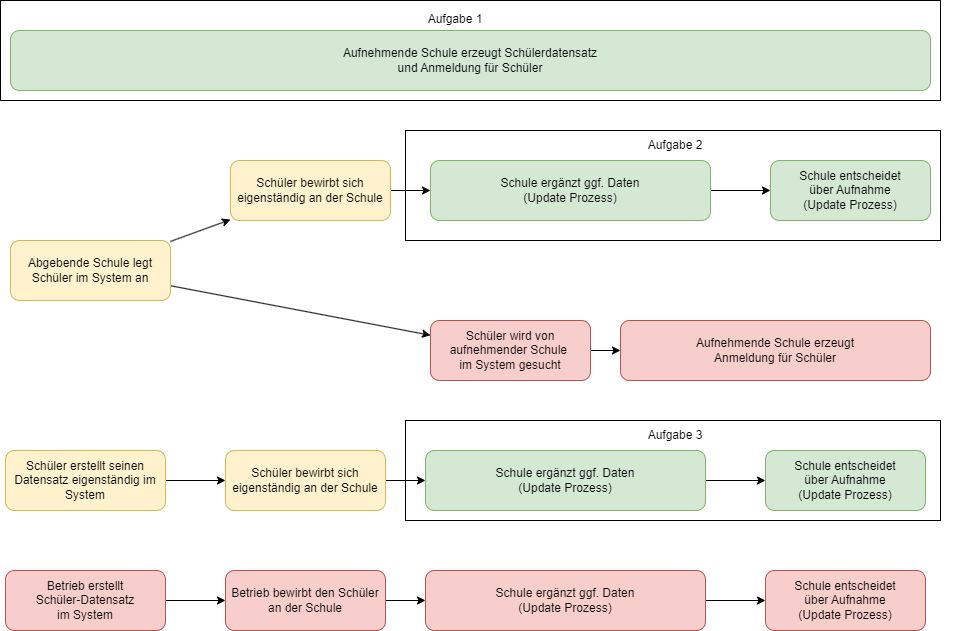
\includegraphics[width=\textwidth]{einordnung-der-aufgaben-in-kontext}
\end{figure}

Für die Durchführung des Feldtests wurden drei spezifische Aufgaben im System entwickelt, die die Teilnehmer während ihrer normalen Arbeitszeit bewältigen sollten. Dabei wurde darauf geachtet, dass die individuellen  Voraussetzungen für die jeweilige Schule gegeben waren, einschließlich  vorhandener Bildungsangebote an der jeweiligen Schule. Die konkreten Aufgaben lauteten wie folgt:

\begin{itemize}
\item Aufgabe 1: \glqq Erstellen Sie bitte für dieses Anmeldeformular von \textit{Max Müller} eine Bewerbung an Ihrer Schule.\grqq{} (Ein Musterexemplar eines solchen Formulars ist Anhang 1 zu entnehmen. Aufgabe 1 macht bisher rund 3,6\% aller erfassten Anmeldungen aus)
\item Aufgabe 2: \glqq Bearbeiten Sie bitte die Bewerbung von \textit{Lotta Meier} nach eigenem Ermessen.\grqq{}  Dieser fiktive Datensatz war so gestaltet, dass die Bewerbung entweder von einer abgebenden Schule oder von der Gemeinde gestellt wurde. Aufgabe 2 macht bisher rund 49,2\% aller erfassten Anmeldungen aus.
\item Aufgabe 3: \glqq Bearbeiten Sie bitte die Bewerbung von \textit{Konrad Schulz} nach eigenem Ermessen.\grqq{}  Bei diesem fiktiven Datensatz wurde die Bewerbung von den Eltern des Schülers eingereicht. Aufgabe 3 macht bisher rund 23,3\% aller erfassten Anmeldungen aus.\footnote{Die Datenquelle der Anteile sind interne Auswertungen des krz.}
\end{itemize}

Andere Anmeldearten sind nicht Gegenstand dieser Untersuchung, da sie zu umfangreich nachzustellen wären. Eine Visualisierung der drei Aufgaben inklusive ihres Kontextes sind in Abbildung \ref{fig:EinordnungAufgaben} ersichtlich. Die rot markierten Aktivitäten werden nicht untersucht. Gelb Markiertes sind vorbereitete Aktivitäten, welche Voraussetzung für die grün markierten zu untersuchenden Aufgabenaktivitäten sind. 

\begin{figure}[H]
    \caption{Übersicht der Aufgabenkonstellationen, gruppiert nach Schulstufe im Rahmen einer Beobachtungs- und Interviewstudie zur Bestimmung der Effektivität und Zufriedenstellung}
    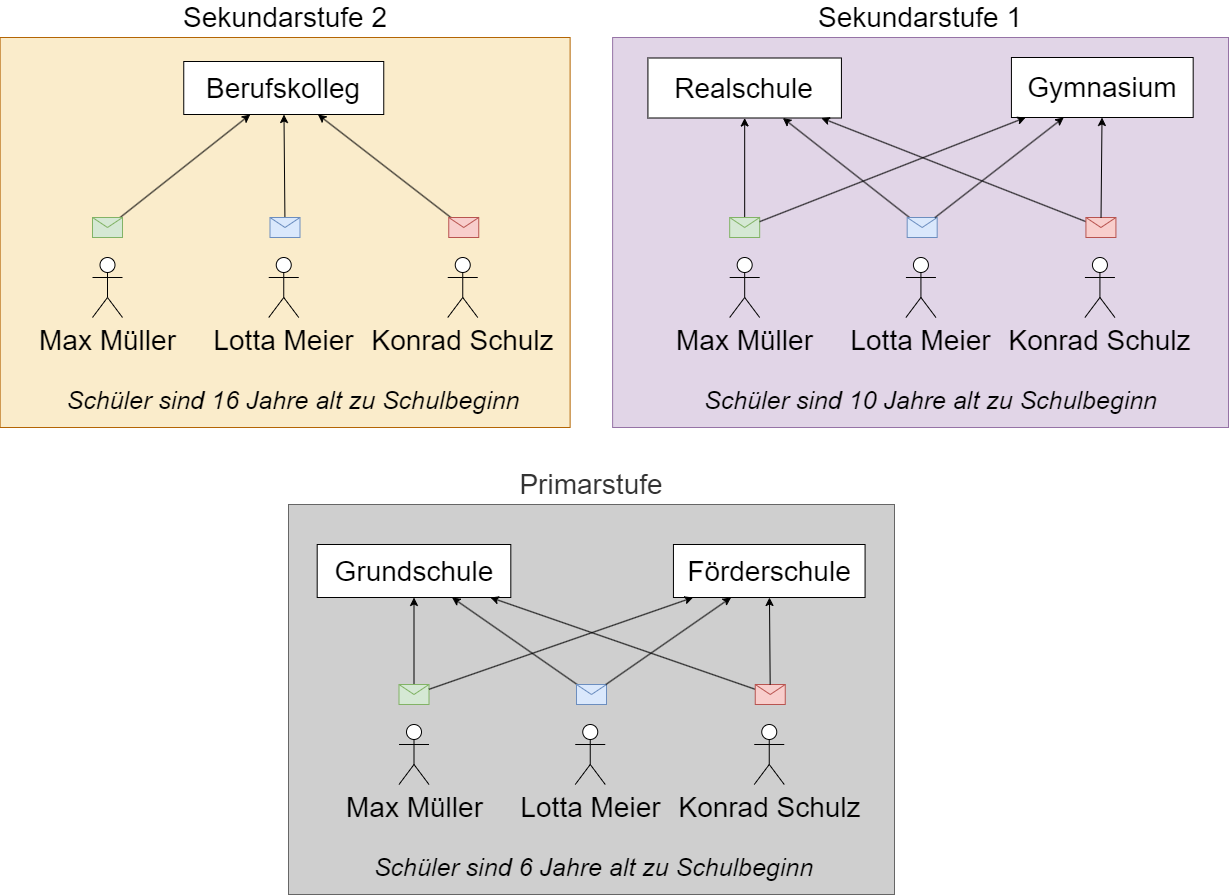
\includegraphics[width=\textwidth]{konstellationenv3}
    \label{fig:konstellationenv3}
\end{figure}

%\begin{figure}[H]
    %\centering
    %\caption{Musteranmeldeformular von der fiktiven Person Max Müller}
    %\begin{adjustbox}{width=\linewidth, center}
        %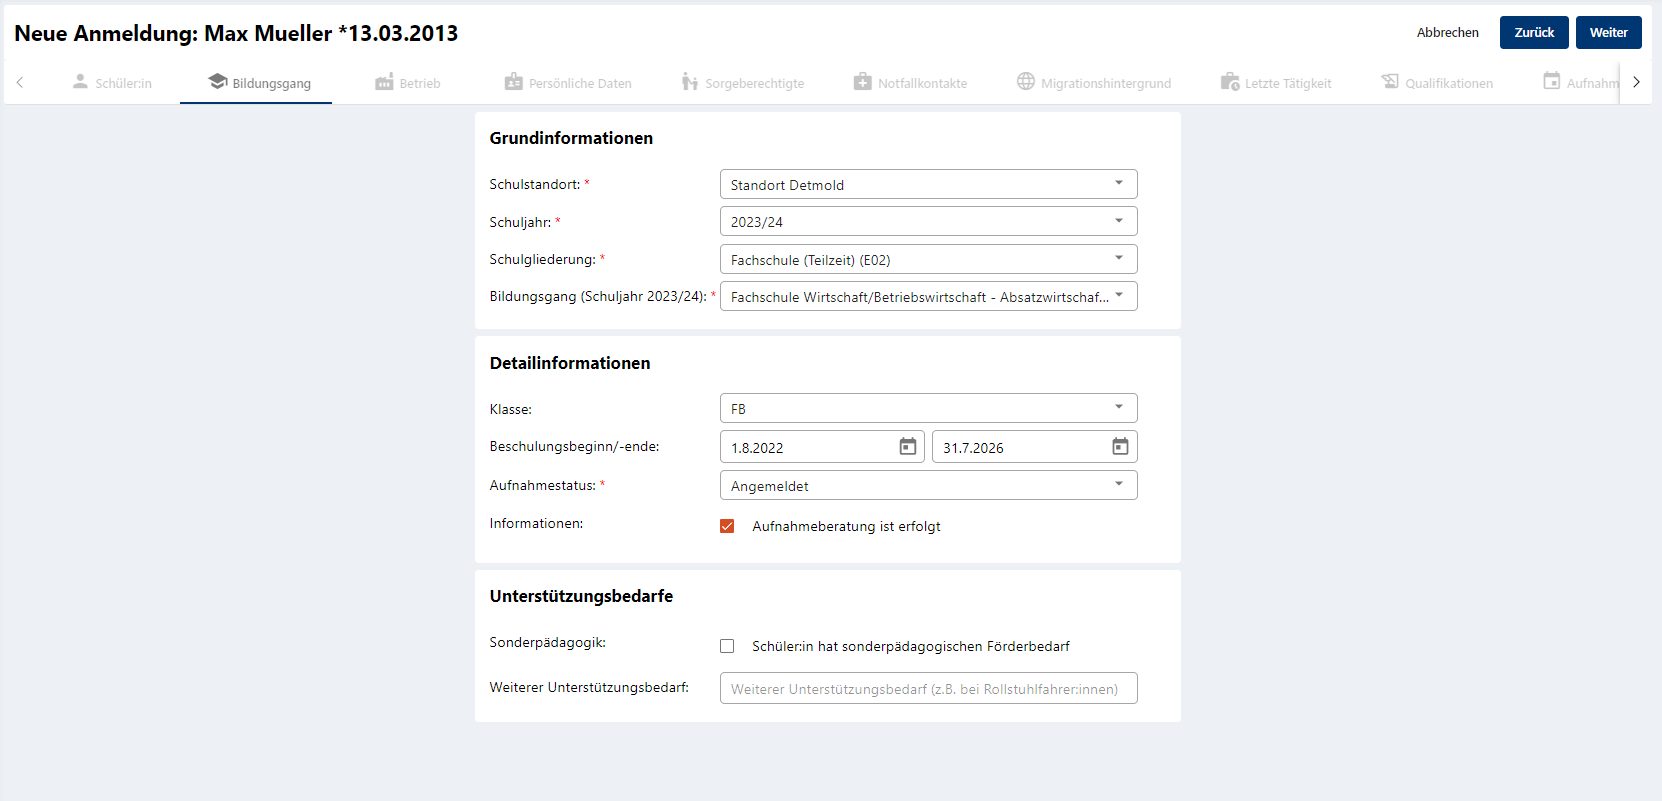
\includegraphics{bildungsgang}
    %\end{adjustbox}
%\end{figure}

Um den Realitätsbezug zu gewährleisten, unterschieden sich die Datensätze je nach Schule, insbesondere in Bezug auf das Geburtsjahr, das an die jeweilige Schulstufe angepasst wurde. So wurde für Bewerbungen an der Primarstufe das Geburtsdatum so gewählt, dass das Schulkind zum Zeitpunkt des ersten Schultages 6 Jahre alt wäre. Im Falle einer Bewerbung für die Sekundarstufe 1 war das Schulkind 10 Jahre und für die Sekundarstufe 2 entsprechend 16 Jahre alt.
Hierzu wurden so genannte Anmeldeformulare der jeweiligen Schule verwendet, die mit Ausnahme des Geburtsdatums und des zu besuchenden Bildungsgangs mit identischen Inhalten ausgefüllt wurden (s. Abbildung \ref{fig:konstellationenv3}).

Zu beachten ist, dass alle Datensätze fiktiv waren, um etwaige Probleme hinsichtlich der Vertraulichkeit zu vermeiden. Dies wurde den Teilnehmern vor Beginn der Aufgaben explizit mitgeteilt.

\subsection{Bereitstellung des Fragebogens}

Im Vorfeld der Untersuchung wurde der Fragebogen den Studienteilnehmern nicht vorab zur Verfügung gestellt. In den initialen Telefongesprächen wurde jedem Teilnehmer ausdrücklich mitgeteilt, dass keine spezielle Vorbereitung für die Teilnahme an der Studie erforderlich sei. Die Software und der Zweck der Studie wurde jedem Teilnehmer in diesem Zuge ebenfalls kurz dargelegt.

Darüber hinaus wurden in diesen Gesprächen die Software \textit{Schüler Online} und der Zweck der Studie den Teilnehmern ausführlich erläutert. Dies gewährleistete, dass jeder Teilnehmer über den Kontext und die Ziele der Studie informiert war und eine Vorstellung von dem hatte, was von ihm oder ihr erwartet wurde.

\subsection{Rollenverteilung während der Studie}

Während der Durchführung der Studie gab es zwei Hauptrollen innerhalb des Forschungsteams: den Interviewer und den Schreiber. Der Interviewer, der die Software mehrere Jahre mitentwickelt hat, war mit den funktionalen Aspekten des Systems gut vertraut, hatte jedoch keine umfangreichen praktischen Erfahrungen hinsichtlich Interviewtechniken. Diese Rolle wurde durch eine Person besetzt, deren Aufgabe es war, die Teilnehmer durch die Aufgaben zu leiten und die Diskussion während des Interviews zu lenken.

Die Rolle des Schreibers wurde durch zwei Personen wahrgenommen, die sich abwechselten. Schreiber A nahm an den Interviews 1 und 4 teil, während Schreiber B an den Interviews 2, 3 und 5 präsent war. Beide Schreiber hatten grundlegende Kenntnisse der Software, die sie während des ersten Jahres ihrer Beteiligung an der Entwicklung der Software erworben hatten.

Die Hauptaufgabe der Schreiber war es, während der Interviews Notizen zu machen und die Reaktionen der Teilnehmer sowie relevante Beobachtungen zu dokumentieren. 

\subsection{Durchführung der Studie}

Die Implementierung der Studie wurde vor Ort in den Schulen durchgeführt. Der Interviewer und der Schreiber trafen sich persönlich mit den Teilnehmern. Beide stellten sich kurz vor und erläuterten den Zweck der zu untersuchenden Software.

Für die Interviews suchten sie sich innerhalb des Raums einen Ort aus, von dem aus sie sowohl den Monitor als auch den Probanden gut beobachten konnten. Während des Interviews stellte der Interviewer sowohl die Fragen aus dem Fragebogen als auch zusätzliche klärende Fragen. Der Notierer hingegen konzentrierte sich hauptsächlich darauf, die Antworten und Beobachtungen zu dokumentieren.

Die Beobachtung der Aufgabenbearbeitung und des Verhaltens der Teilnehmer war sowohl dem Interviewer als auch dem Notierer zugeordnet. Um ein realistisches Szenario zu gewährleisten, wurden keine fachlichen Rückfragen der Studienteilnehmer beantwortet - sie mussten sich, ähnlich wie in einer realen Arbeitsumgebung, auf die Dokumentation und ihre eigenen Ressourcen verlassen.

Den Teilnehmern wurde versichert, dass das Ziel der Studie war, die Software und nicht den Anwender zu testen. Das Interview und die Beobachtung fanden gleichzeitig statt und dauerten zwischen einer und drei Stunden.

Die Teilnehmer agierten entsprechend des \textit{Meister-Schüler-Modells} in der Rolle des Meisters, von denen der Schüler (Interviewer) lernen kann.\cite{Seibert-Giller,jacobsen} Sie wurden dementsprechend nicht in ihren Ansichten korrigiert.

Um in dieser Ausarbeitung die Antworten und Beobachtungen zuordenbar zu machen, sind die Resultate der Sekretärinnen des Gymnasiums (1), der Realschule (2), der Förderschule (3), der Grundschule (4) und des Berufskollegs (5) konsequent und analog zu ihrer Indexziffer den Anhängen \ref{section-InterviewGymnasium} - \ref{section-InterviewBerufskolleg} zugeordnet.

In der ersten Durchführung mit dem Gymnasium (1) gab es die Besonderheit, dass  in Anlehnung an die Empfehlung des Leitfaden Usability ein erfahrener Requirements Engineer (der Product Owner der Software) mittels Anruf zugeschaltet wurde, der \glqq in Form einer Supervision die Gesprächssituation beobachtet, bewertet und anschließend mit dem Beobachteten [besprochen hat]\grqq{}\cite{dakks}.

In drei Fällen (Gymnasium (1), Realschule (2) und zeitweise bei der Förderschule(3)) waren bei der Durchführung der Interviews zwei Mitarbeiter vonseiten der Studienteilnehmer anwesend. Es wurde die Entscheidung getroffen, das Interview nur mit dem vorab rekrutierten Teilnehmer durchzuführen. Kommentare und Diskussionen zwischen den Mitarbeitern waren jedoch zulässig, um ein realistischeres Szenario zu belassen. Die gesammelten Daten wurden ausschließlich aus den Ansichten, Antworten und Beobachtungen des Interviewpartners erfasst, nicht von dem weiteren Mitarbeiter. Die Interviews wurden direkt in Microsoft Word dokumentiert. Es wurden keine Audio- oder Filmaufnahmen erstellt.

\subsection{Nachbereitung und Auswertung der Studie}

Unmittelbar nach Abschluss der Interviews wurde eine erste Nachbearbeitung der gesammelten Daten durchgeführt. Hierbei wurden unklare oder zu kurz formulierte Notizen präzisiert und ausführlicher beschrieben. Es ist wichtig zu betonen, dass diese Nachbearbeitung nur für Einträge vorgenommen wurde, bei denen eine eindeutige Interpretation möglich war. Bei Notizen, bei denen das Potenzial für Fehlinterpretationen bestand oder die im Nachhinein unklar blieben, wurden keine Änderungen vorgenommen. Sie wurden in ihrer ursprünglichen Form beibehalten, um die Möglichkeit von Missverständnissen zu minimieren.

Für die Auswertung der gesammelten Daten wurden keine speziellen Analysetools oder ähnliche Instrumente verwendet. Die Auswertung erfolgte lediglich bei den Notizen, die unmissverständlich waren und bei denen man keine Fehlinterpretationen beim Ausformulieren machen konnte. Bei Punkten, die potenziell fehlinterpretiert werden konnten oder im Nachhinein unklar waren, wurden keine Ausformulierungen durchgeführt, sondern die Notiz so belassen wie sie mitgeschrieben wurde. Verständnis der Benutzererfahrungen und -bedürfnisse zu gewinnen.

%todo: Die Ergebnisse der unterschiedlichen Schulen wurden jedoch händisch miteinander auf Gemeinsamkeiten und Kontroversen verglichen. 


\subsection{Materialien und Ressourcen}

Für die Durchführung der Studie war vonseiten der Teilnehmer lediglich ein Computer mit Internetzugang erforderlich, um den Zugriff auf die Anwendung zu ermöglichen. Darüber hinaus war kein zusätzliches Material notwendig.
Vonseiten der Moderation wurden ein Laptop für Notizen und der ausgearbeitete Fragebogen sowie die Anmeldeformulare verwendet

%  Ethik: Welche ethischen Gesichtspunkte wurden bei der Durchführung des Interviews berücksichtigt, z.B. in Bezug auf Datenschutz oder Anonymität?
 
 
% In diesem Kapitel solltest du die Methoden und Techniken, die du zur Durchführung deiner Projektarbeit verwendest, beschreiben und begründen. Hier sollten auch die Einzelheiten zur Durchführung des leitfadengestützten Interviews enthalten sein.
% Für das leitfadengestützte Experteninterview solltest du in der Methodik deiner Projektarbeit den Ablauf und die Durchführung des Interviews beschreiben. Hierbei sollst du beispielsweise folgende Punkte erwähnen:
% Teilnehmer: Wer wurde für das Interview ausgewählt und warum? Wie viele Experten wurden befragt? 

% material
% Wie haben wir den Fragebogen erstellt? 
% Schulleiter zeigt nochmal weitere Aspekte auf
% Offene Fragen gemacht => Warum offene Fragen
% induktives vorgehen
% ich habe jedes Sekretärin vorher telefonisch gesprochen

% Fragebogen ist delegiert ans Team und ein Zwischenergebnis. Ist ein Ergebnis eines Expertenteams für dieses Programm
% Experten sind Material


% ggf. der fixierte Nutzungskontex 
\section{Ergebnisse}
%In diesem Kapitel solltest du die Ergebnisse deiner Projektarbeit ausführlich und detailliert darstellen. Hierbei solltest du auch das Ergebnis des leitfadengestützten %Interviews einbeziehen.
%
%Expertenmeinungen: Was waren die Meinungen und Einschätzungen der befragten Experten zu deinem Thema?
%Unterschiede und Gemeinsamkeiten: Gab es Unterschiede oder Gemeinsamkeiten in den Antworten der Experten? Gab es übereinstimmende Aussagen oder Diskrepanzen?
%Erkenntnisse: Welche Erkenntnisse konntest du aus den Antworten der Experten gewinnen? Wie tragen die Ergebnisse zu deiner Forschungsfrage und zum aktuellen Stand der Forschung %bei?

%Screenshots des untersuchten Prozesses der Anwendung

\subsection{Identifizierter Nutzungskontext}

% Benutzer:
%     - Kenntnisse: 
%     - Fertigkeiten:     
%     - Erfahrungen:    
%     - Ausbildiungen:     
%     - physische Merkmale:     
%     - Gewohnheiten:   
%     - Vorlieben:    
%     - Fähigkeiten: 
%     - Alter: 
%     - Geschlecht: 
%     - Bildungsniveau: 
%     - Sprachkenntnisse: 
%     - Kultureller Hintergrund: 
%     - Berufliche Erfahrungen: 
%     - Hobbies und Interessen: 
%     - Körperliche Einschränkungen: 
%     - Krankheiten oder Behinderungen: 
% Aufgaben:
%     - Die Art, wie der Benutzer die Aufgabe ausführt
%     - Häufigkeit
%     - Zeitdauer
%     - Priorität der Aufgabe
%     - Komplexität der Aufgabe
%     - Fehleranfälligkeit
%     - Abhängigkeit von anderen Aufgaben
%     - Auswirkungen auf andere Aufgaben

% Ausrüstung:
%     - Hardware
%     - Software
%     - Materialien
%     - Beleuchtung
%     - Möbel
%     - Raumgestaltung
% Verfügbarkeit der Ausrüstung
% Qualität und Zustand der Ausrüstung
% Einfachheit der Bedienung der Ausrüstung
% Kompatibilität der Ausrüstung mit anderen Geräten oder Software
% Umgebung: 
%     - Physischen
%     - sozial 
%     - kulturell: Arbeitsweisen und Einstellungen
%     - organisationsbezogen 
    

% Beschreibe in den qualitativen Ergebnissen für jeden Abschnitt:

% erst allgemeine, dann detaillierte Ergebnisse
% wiederkehrende Muster
% signifikante oder repräsentative individuelle Antworten
% relevante Zitate aus den Daten
% keine Interpretationen oder Spekulationen


Die Studienteilnehmer haben die Aufgabe 2 und 3 ("Bearbeiten Sie bitte die Bewerbung von 'Lotta Meier' nach eigenem Ermessen" sowie "Bearbeiten Sie bitte die Bewerbung von Konrad Schulz nach eigenem Ermessen") anhand der Informationslage nicht erfolgreich abgeschlossen, da der Anmeldestatus bei allen Studienteilnehmern auf "angemeldet" verblieben ist. Der Anmeldestatus hätte zwingend einen der Status "Aufgenommen", "Warteliste", ""

Die Verbindungsgeschwindigkeit variierte gemäß der Angaben der Teilnehmern sowie den Beobachtungen von hinreichend schnell im Sinne von "Jede Seite und jeder Inhalt lädt innerhalb von unter einer Sekunde vollständig" bis zu langsam im Sinne von: "Der initiale Seitenaufbau dauert länger als 20 Sekunden". Konsekutive Seitenaufrufe waren aufgrund der Architektur der Software schneller (Single Page Application - schnelles Rendering der Folgeseiten in weniger als einer Sekunde), es kam noch zu geringfügigen Ladezeiten (weniger als drei Sekunden) bei Dropdown Feldern und Listen, wo Daten nachgeladen werden mussten.
\section{Diskussion}
%In diesem Kapitel solltest du deine Ergebnisse diskutieren und in den Kontext der Literatur und des aktuellen Forschungsstandes einordnen. Hier kannst du auch Schwächen und %Limitationen deiner Projektarbeit besprechen und einen Ausblick geben, wie weiterführende Forschung aussehen könnte.

%Grobstruktur für einen Evaluationsbericht (vgl. Skript)
%Fotos der Umgebung / des Arbeitsplatzes?

% laut janna erst positives und negatives im allgemeinen der studie
% danach ergebnisse interpretieren stück für stück, immer wieder auf theorie (den kriterienkatalog) beziehen
% endfazit: Leitfragen final beantworten
% Ausblick

Positives: Die Art der Studie war richtig gut gewählt. Durch den qualitativen Charakter der Studie konnten viele Erkenntnisse gewonnen werden, welche Aspekte Nutzer die Zufriedenstellung des Nutzers mindern oder sie daran hindern, ihre Aufgaben effektiv zu bewältigen. 
Negatives: Die Repräsentativität der Studie kann aufgrund des relativ geringen Stichprobenumfangs von 5 untersuchten Teilnehmern als nicht ausreichend betrachtet werden. Dies war allerdings wie auch in der Einleitung genannt nicht das Ziel der Studie. 
Darüber hinaus war die Studie insofern nicht realitätsgetreu, alsdass keine Echtdaten verwendet wurden und auch nicht im echten Arbeitskontext gearbeitet wurde. Dies hätte einen anderen Zeitpunkt (außerhalb der Sommerferien) und Erklärungen sowie Vorkehrungen zur Sorgfaltspflicht bezüglich Datenschutz noch erforderlich gemacht, wurde allerdings bewusst nicht gemacht, da sonst neben ebenjener Sorgfaltspflicht mit erheblichen Unterbrechungen hätte gerechnet werden müssen, die möglicherweise zum Misserfolg von den Untersuchungen gefolgt hätten. Es ist eine Abwägung, ob man es als Leser dieser Studie hinnehmbar betrachtet, dass die Sekretärin basierend auf Erfahrungen davon berichtet, wie sie in der Praxis störende Einflüsse wie beispielsweise Unterbrechungen behandelt.


\subsection{Hawthorne Effekt}
Der Hawthorne-Effekt besagt, dass Personen ihr Handeln verändern, weil sie wissen, dass sie unter Beobachtung stehen. Er kann bei Teilnehmenden an wissenschaftlichen Experimenten vorkommen, deren Verhalten beobachtet wird. So ist ihr Verhalten unnatürlich.

\subsection{ggf. Soziale Erwünschtheit}
\grqq{} Beim Effekt der sozialen Erwünschtheit verändern Teilnehmende ihr Verhalten oder ihre Antworten bei Fragebogen, um ein positives Bild von sich selbst abzugeben.\glqq 

\subsection{DECIDE Ansatz}
\subsection{Beobachtung}
\subsection{Hawthorne Effekt}
\subsection{Loud Thinking}
\subsection{Feldtest / Labortest}

-Soziale Erwünschtheit
-Mein Schreiberling: Muss er ungelernt oder gelernt sein? Vergleich mit Literatur
-Hawthorne Effekt
Der Hawthorne Effekt könnte vermieden werden, indem man diese Studie als eine Stille Beobachtung durchführt. 
%

Die Aufgaben 2 und 3(\glqq Bearbeiten Sie bitte die Bewerbung von \textit{Lotta Meier} nach eigenem Ermessen\grqq{} sowie \glqq{} Bearbeiten Sie bitte die Bewerbung von \textit{Konrad Schulz} nach eigenem Ermessen\grqq{}) hätten anders formuliert werden müssen oder in einen anderen Kontext gesetzt werden können. Es wurde sich in der Studie jedoch bewusst dazu entschieden, die Aufgabe sehr offen zu formulieren, da geprüft werden sollte, wie die Studienteilnehmer mit der Situation umgehen würden, da in der Realität auch nur diese Bewerbung vorliegen wird - ohne konkrete Handlungsanweisung. In der Software wird nur von \glqq unbearbeiteten Bewerbungen\grqq{} gesprochen. Es besteht die Möglichkeit, dass das Ergebnis anders ausfällt, wenn die Studienteilnehmer in einem anderen zeitlichen Kontext gearbeitet hätten, da zum Zeitpunkt der Durchführung der Studie keine Aufnahmephase an dieser Schule bestand - die regulären, echten Bewerbungen für das fragliche Schuljahr wurden allesamt bereits im Februar bearbeitet. Sie hatten somit keinen intuitiven intrinsischen Drang, akut über Aufnahmeentscheidungen zu beurteilen. Aber auch der Fakt, dass in einigen Durchführungen der Anmeldestatus \glqq Angemeldet\grqq{} fälschlicherweise als \glqq Aufgenommen\grqq{} missinterpretiert wurde, kann hierfür eine Ursache gewesen sein.
Die Studienergebnisse sind an einigen Stellen möglicherweise verfälscht. Wenn man diese Studie zu einem anderen Zeitpunkt wiederholen würde (zu einem Zeitpunkt der Anmeldephase) würden die Ergebnisse teilweise anders ausfallen. Beispiele wären hier zu nennen die Auswahl des Schuljahres, die Auswahl der Klasse sowie inbesondere der Aufnahmestatus. Aufgrund dessen wäre also eine Wiederholung der Untersuchung ratsam und eine Überprüfung, inwiefern die Ergebnisse anders ausfallen.

Viele Ergebnisse sind deckungsgleich gewesen
Der Stichprobenumfang von 5-6 Studienteilnehmern ist sehr gering. Es war jedoch nicht das Ziel der Forschung, da man erste Eindrücke gewinnen . Es kann nicht davon ausgegangen werden, dass die Ergebnisse repräsentativ für ganz Nordrhein-Westfalen sind. Hierzu müsste eine quantitative Forschung mit einem größeren Stichprobenumfang erfolgen, um die Ergebnisse zu validieren oder zu falsifizieren.
Reliabilität wurde insofern sichergestellt, alsdass die Fragebögen identische Fragen beinhalteten. 

Der Leitfaden Usability wurde zurückgezogen, es gibt jedoch keine aktuellere Version

Aufgrund der Unerfahrenheit des Interviewers könnten Interpretationsfehler und Bias vorliegen. Auch hätte ein erfahrener Interviewer möglicherweise bessere Rückfragen gestellt, damit die Fragen adäquat beantwortet werden.

Der Stichprobenumfang ist zu gering um von einer repräsentativen Darstellung zu sprechen. Dies war allerdings auch nicht das Ziel der Studie


Fragebogen: Es wurde festgestellt, dass weitere Fragen hätten nach der Durchführung gestellt werden sollten, da der Studienteilnehmer dann die ein oder andere Frage präziser hätte beantworten können.
Die Frage \glqq Welche Arbeitsschritte sind durchzuführen\grqq{} regt etwas zu Spekulation an, welche Schritte im Prozess kommen werden. Es wurde allerdings in den Interview rückbezogen auf den Sinn der Frage, dass eine ganzheitliche und übergreifende Betrachtung des Prozesses erwünscht ist.
Auch die Frage \glqq Welche Ergebnisse / Teilergebnisse entstehen und wie werden diese ggf. verwertet / weitergeführt?\grqq{} lädt zu Spekulationen ein, wenn sich die Teilnehmer auf die Software beziehen. Sofern sich auf die bisherigen Papierbewerbungen bezogen wird, wie es auch gewollt war, sind es verwertbare Ergebnisse.

Alleinstellungsmerkmal der Bildungsangebote bei Berufskollegs, da es hier mehrere gibt anstatt nur eins oder 2 wie bei anderen Schulen. Dort ist die Auswahl des Bildungsgangs trivial.

Generell
- Es wurde oft nicht verstanden, welche Felder Pflichtfelder sind. 2 hatte dies beim Beschulungsbeginn moniert, 5 hatte gefragt \glqq Die roten Felder sind Pflicht oder? ist das irgendwo erklärt?\grqq{}. 3 hat das Sternchen neben dem Labeltext als Pflichtfeld interpretiert. 3 hatte beim ID-Schlüssel aber zuvor nur vermutet, dass der nicht erforderlich sei. 1 hatte bei der Klasse länger verweilt, da zwar keine auswählbare Klasse vorhanden war, das Feld war allerdings kein Pflichtfeld. Insgesamt wurde also nur teilweise  erkannt, dass das Sternchen neben dem Label das zugehörige Feld als Pflichtfeld deklariert.



>Beschreiben Sie die Ausgangssituation die vorliegt, bevor Sie die Aufgabe \glqq Bewerbung eines Schülers\grqq{} durchführen.


Bzgll. Ausgangssituation:
Die Wichtigkeit von Zwischenarbeit mit den Eltern variiert. Bei den Berufskollegs werden sie teilweise nicht mal angefordert als Sorgeberechtigte, wenn die Schüler älter als 18 sind, wohingegen es bei Förderschulen sehr wichtig ist.
Wenn Anmeldedaten schriftlich erfolgen sind diese anfällig für unleserliche Schrift oder ungültige Daten. Das sollte mit einer digitalen Erfassung, mitunter auch durch Plausibilitätsprüfungen an geeigneten Stellen vermieden werden können. Dieses Problem wird dementsprechend obsolet. Wissentliche Falschangaben sind schwierig überprüfbar, sollten allerdings auch versucht werden zu berücksichtigen. Hier könnte eine enge Kommunikation mit der abgebenden Schule oder der Kommune erforderlich sein.



Bzgl. Schüler Tab: Es gibt zwar eine Erklärung für ID-Schlüssel, die hat jedoch keiner wahrgenommen oder nach lesen ebenjener das Feld verstanden. Die aktuelle Lösung ist in der aktuellen Form ungenügend. Es liegt hier keine Freiheit von unmissverständlichen Feldern vor.

Bzgl. Bildungsgang Tab:
Eine Vereinheitlichung des Prozesses sollte in Betracht gezogen werden. Sowohl die Reihenfolge könnte sich an \textit{SchILD} anlehnen als auch die Begrifflichkeiten wie Neuaufnahme, damit eine einheitlicher unmissverständlicher Jargon vorliegt
Inbesondere die Bedeutungen der Aufnahmestatusse wurden gravierend missverstanden. Dies hat fatale Folgen auf die Erwartungshaltung und Rechtsansprüche der Schüler, da eine Schüler, der beispielsweise bei einer Anmeldung fälschlicherweise den Status \textit{Aufgenommen} erhält, eine rechtliche Zusage der Schule erhält, dass der Schüler dort lernen darf. Hier ist es dringend notwendig, die Begrifflichkeiten klar und unmissverständlich zu definieren, sodass die Erwartungen des Schulpersonals nach Rechtssicherheit erfüllt werden können. Laut 2 würden die Eltern so einen Nachweis der Aufnahme als \glqq Druckmittel\grqq{} verwenden, hier gebe es laut ihr auch einen starken Elternwillen.
Ein weiteres Beispiel aus der Untersuchung:  1 hatte den Status Warteliste missverstanden und als \glqq In Bearbeitung\grqq{} interpretiert. Warteliste wird allerdings von der Anwendung mehr im Sinne von nachrückenden Personen gehandhabt, falls aufgenommene Schüler ihre Anmeldung zurückziehen. 5 hätte Erklärtexte erwartet. 

Bzgl. Persönliche Daten Tab:
Es fehlt eine Funktionalität, die es ermöglicht, dass man Postleitzahl-Ort Kombinationen auch findet, wenn man zunächst den Ort eintippt, anstatt mit der Postleitzahl zu beginnen. Mehrere Sekretärinnen hatten versucht, mittels der Eingabe des Ortes die Kombination aus PLZ und Ort im Dropdown zu finden.

Bzgl. Sorgeberechtigten Tab:
Bezüglich des Feldes Feld Adressart: der Eingabefluss ist nicht intuitiv. Es erfolgen Ein-und ausblendelogiken basierend auf der Adressart für das System, allerdings auf kosten der Nutzerführung. Dies ist nicht nutzerzentriertes Verhalten der Anwendung, sondern systemzentriert. 

Bzgl. Notfallkontakte Tab:
4 hatte missinterpretiert, wozu die Notfallkontakte dienen. Sie dachte sie würde den Sorgeberechtigten weitere Informationen anreichen, dabei dienen die Notfallkontakte dazu, weitere Kontakte wie Oma, Onkel, Schwester oder Freunde der Familie (vertraute Personen im allgemeinen) einzutragen, falls ein Kind beispielsweise in der Schule verunfallt und die Sorgeberechtigten nicht erreichbar sind.

Bzgl. Letzte Tätigkeit
3 fand den Tab \glqq Letzte Tätigkeit\grqq{} \glqq sinnlos\grqq{}. Dieser Tab dient der Schulpflichtsüberwachung, diesen Zweck konnte sie jedoch nicht eigenständig erkennen.

Bzgl. Bemerkungen
Bei den Bemerkungen lagen (mitunter folgenschwere) Interpretationsschwierigkeiten und -fehler vor. Wenn der Anwender nicht versteht, welche Felder für die Eltern und Schülern sichtbar sind, laufen sie Gefahr, dass sie interne Informationen, die sie eigentlich für sich behalten wollen, unbewusst ebenjenen zugänglich machen. 

Bzgl. Update
Die \glqq Anmeldung wurde exportiert\grqq{} Checkbox auf dem Reiter \glqq Bewerbung\grqq{} hätte besser erklärt werden müssen, da 1,2,3 Verständnisschwierigkeiten hatten oder diese Felder fehlinterpretiert hatten.

Bzgl. Wie verständlich waren die Rückmeldungen der Anwendung?
Es kam vermehrt vor, dass eine Fehlermeldung beim Speichern einer Anmeldung auftrat. Hier gab es dann allerdings oft keinen Hinweis, wo der Fehler vorlag. Dies beruhte auf einer fehlerhaften Funktionalität der Anwendung, grundsätzlich existiert diese Funktionalität. Wenn ein Feld als fehlerhaft markiert wurde, wurde diese Funktionalität gelobt.

Es sollte Interpretation- und Wiedererkennungseffekte geben. Beispielsweise sollte das Sternchen neben den Labels immer interpretiert werden als Pflichtfeld. Autocomplete-Felder sollten als solche immer wahrgenommen werden können.

Zufriedenstellung und Effektivität:
1 und 4 waren überfordert damit, auf die korrekte Seite zu navigieren. Es scheint, dass die Navigation und Strukturierung innerhalb der Software für die Nutzer nicht intuitiv und selbsterklärend ist. Dies hat merklich zu einer nichterreichung der Erwartungen an die Software geführt. Es lag in dem Sinne eine aus dem Theorie-Kapitel definierten Behinderung vor. 
Damit die Sekretärin 5 eine Bewerbung erfolgreich abschließen kann, muss der zuständige Lehrer in die Aufnahmeentscheidung eingebunden werden. Dies würde eine Einbindung ebenjener erforderlich machen.



%\appendix
%
\newpage
\section{Anhang}

\subsection{Musteranmeldeformular}
\begin{figure}[H]
    \centering
    \caption{Musteranmeldeformular von der fiktiven Person Max Müller}
    \begin{adjustbox}{height=0.85\textheight, center}
        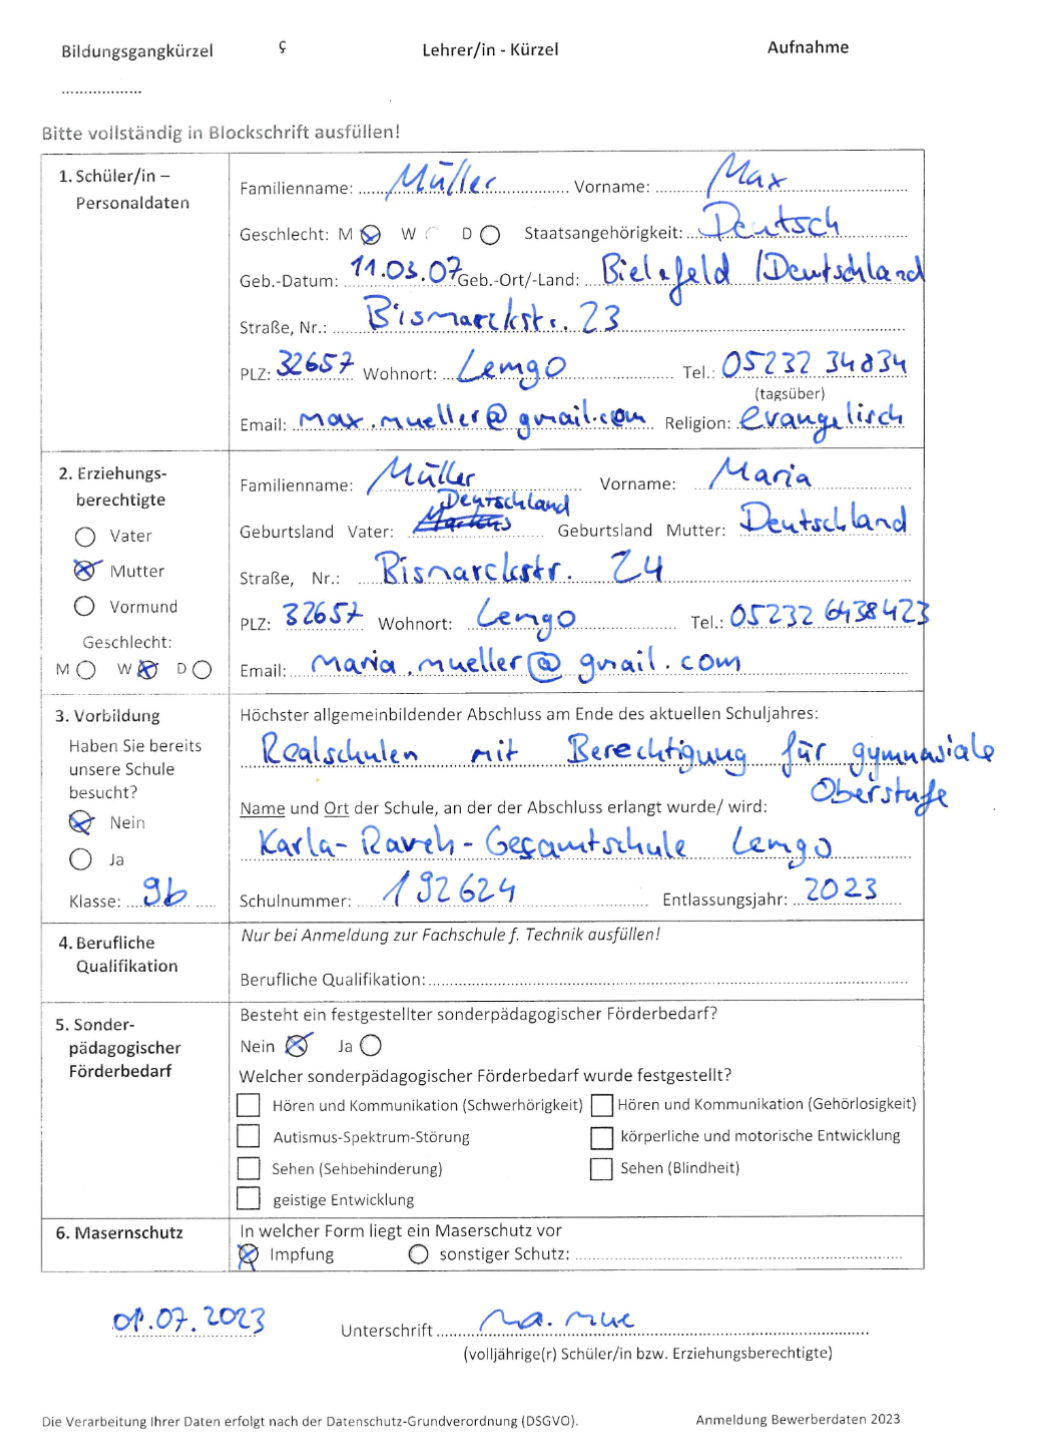
\includegraphics{bewerbungsformular1}
    \end{adjustbox}
\end{figure}

\begin{landscape}

    \begin{longtable}{p{15cm}cc}
        \caption{Your Table} \label{tab:mytable} \\
        \toprule
        Erfordernis & Beispiel & Zugehörige Ergebnisse \\
        \midrule
            Der Benutzer muss inkorrekte Daten identifizieren und korrigieren können. & a & E1, E2 \\
            Der Benutzer muss die an ihn eingereichten Formulare korrekt übertragen können. & a & E5, E6 \\
            Der Benutzer muss unzulässige Bewerbungen identifizieren können. & a & E9, E10 \\
            Der Benutzer muss die Daten datenschutzkonform in die Anwendung eintragen können und über mögliche Verstöße informiert werden. & a & E11 \\
            Der Benutzer muss erkennen können, wie er zum korrekten Prozess gelangt. & a & E12 \\
            Der Benutzer muss bezüglich Aufnahmeentscheidungen mit den Entscheidungsträgern zusammen arbeiten können. & a & E7, E8 \\
            Der Benutzer muss die Software auch bei fehlenden Daten bedienen können.  & a & \\
            Der Benutzer muss Aufnahmekriterien berücksichtigen können. & a & \\
            Der Benutzer muss Termine für Aufnahmeberatungsgespräche hinterlegen können. & a & b \\
            Der Benutzer muss Schülerakten erzeugen können. & a & b \\
            Der Benutzer muss Daten aus anderen Programmen übernehmen können. & a & b \\
            Der Benutzer muss Adressrecherchen durchführen können. & a & b \\
            Der Benutzer muss eine Kurzanleitung für den Einstieg abrufen können. & a & b \\
            Der Benutzer muss die Software auch bei fehlenden Daten bedienen können. & a & b \\
            Der Benutzer muss innerjährige Wechsel und Stufenwiederholungen erfassen können. & a & b \\
            Der Benutzer muss langfristige Beurlaubungen vermerken können. & a & b \\
            Der Benutzer muss auch komplizierte Bewerbungen und Sonderfälle bearbeiten können. & a & b \\
            Der Benutzer muss seinen bisherigen Jargon verwenden können. & a & b \\
            Der Benutzer muss die Aufgaben und Prozesse intuitiv bedienen können. & a & b \\
            Der Benutzer muss eine Adressvalidierung vornehmen können. & a & b \\
            Der Benutzer muss Erreichbarkeiten von Notfallkontakten erfassen können. & a & b \\
            Der Benutzer muss unterschiedliche Arten von Notfallkontakten erfassen können. & a & b \\
            Der Benutzer muss erkennen können, ob ein Schüler volljährig ist. & a & b \\
        \endfirsthead
        \toprule
        Erfordernis & Beispiel & Zugehörige Ergebnisse \\
        \midrule
        \endhead
        \bottomrule
        \endfoot
            Der Benutzer muss Nachweise über das Sorgerecht hinterlegen können. & a & b \\
            Der Benutzer muss Daten auch bei Programmabbrüchen wiederherstellen können. & a & b \\
            Der Benutzer muss ähnliche Datenabfragen aus vorherigen Formularen übernehmen können. & a & b \\
            Der Benutzer muss bei Bedarf Handbücher heranziehen können. & a & b \\
            Der Benutzer muss bei Bedarf Fachterminologie nachschlagen oder verstehen können. & a & b \\
            Der Benutzer muss jederzeit darüber Bescheid wissen, welche Daten den Eltern und Schülern angezeigt werden. & a & b \\
            Der Benutzer muss den Systemstatus jederzeit einsehen können. & a & b \\
            Der Benutzer muss Bewerbungslisten in geeigneter Form exportieren können. & a & b \\
            Der Benutzer muss Daten in Schulverwaltungsprogramme wie Schild exportieren können. & a & b \\
            Der Benutzer muss Daten nach Excel exportieren können. & a & b \\
            Der Benutzer muss Berichte anfertigen können. & a & b \\
            Der Benutzer muss Anmeldezeiträume berücksichtigen. & a & b \\
            Der Benutzer muss mit anderen Behörnden zusammenarbeiten können. & a & b \\
            Der Benutzer muss über Änderungen an Bewerbungen regelmäßig informiert werden. & a & b \\
            Der Benutzer muss zusätzliche Informationen zu einer Bewerbung hinterlegen können. & a & b \\
            Der Benutzer muss Dokumente ausdrücken können. & a & b \\
            Der Benutzer muss Dokumente digitalisieren und beim Datensatz hinterlegen können. & a & b \\
    \end{longtable}




\subsection{bildungsgang}
\begin{figure}[H]
    \centering
    \caption{Testüberschrift}
    \begin{adjustbox}{width=\linewidth, center}
        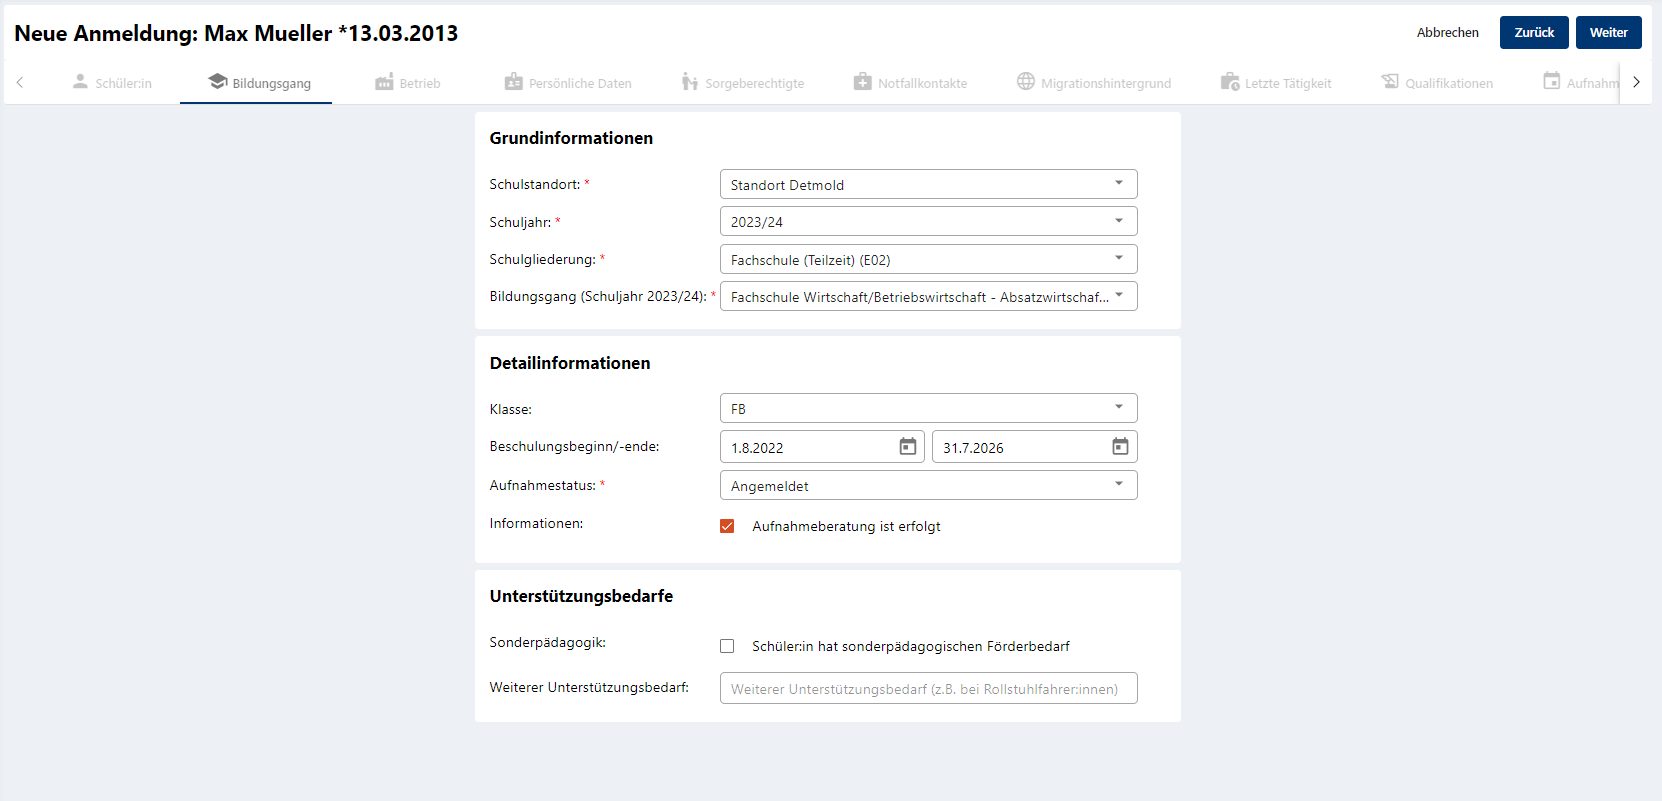
\includegraphics{bildungsgang}
    \end{adjustbox}
\end{figure}

\subsection{sorgeberechtigte-liste}
\begin{figure}[H]
    \centering
    \caption{Testüberschrift}
    \begin{adjustbox}{width=\linewidth, center}
        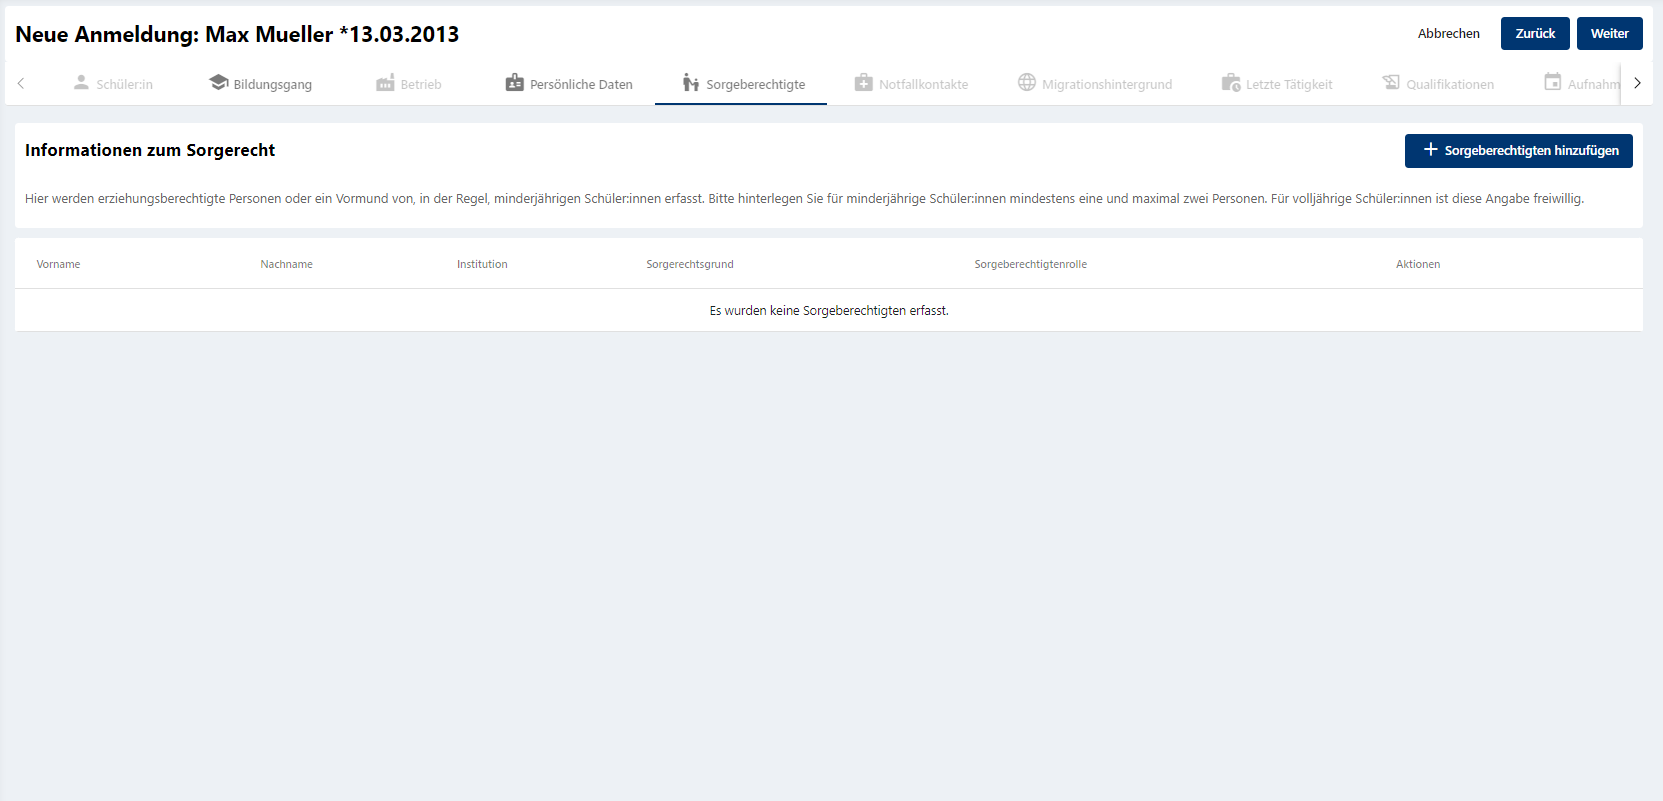
\includegraphics{sorgeberechtigte-liste}
    \end{adjustbox}
\end{figure}

\subsection{sorgeberechtigter-person}
\begin{figure}[H]
    \centering
    \caption{Testüberschrift}
    \begin{adjustbox}{width=0.5\linewidth, center}
        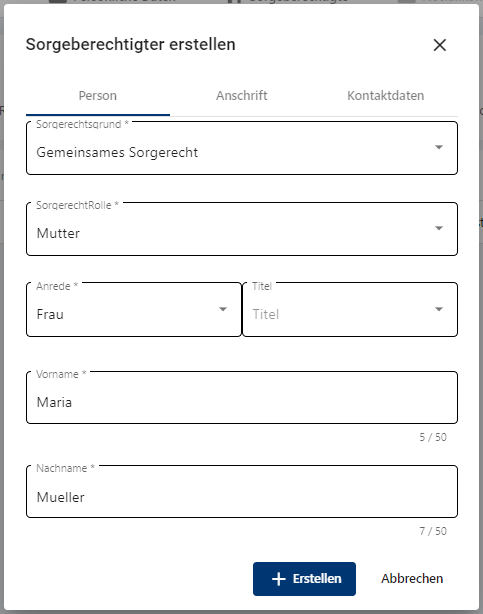
\includegraphics{sorgeberechtigter-person}
    \end{adjustbox}
\end{figure}

\subsection{sorgeberechtigter-anschrift}
\begin{figure}[H]
    \centering
    \caption{Testüberschrift}
    \begin{adjustbox}{width=0.85\linewidth, center}
        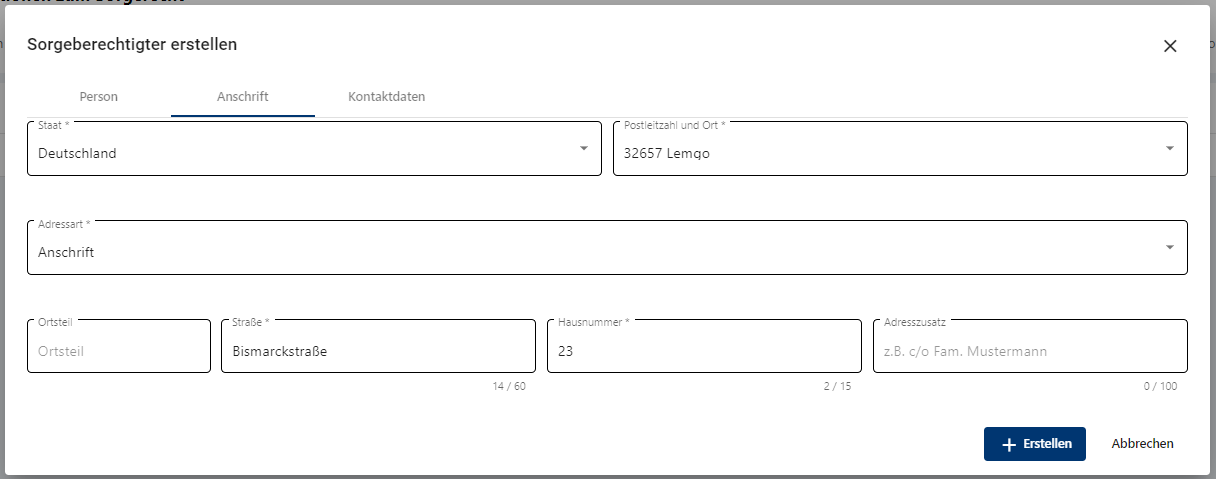
\includegraphics{sorgeberechtigter-anschrift}
    \end{adjustbox}
\end{figure}

\subsection{sorgeberechtigter-kontakt}
\begin{figure}[H]
    \centering
    \caption{Testüberschrift}
    \begin{adjustbox}{width=0.6\linewidth, center}
        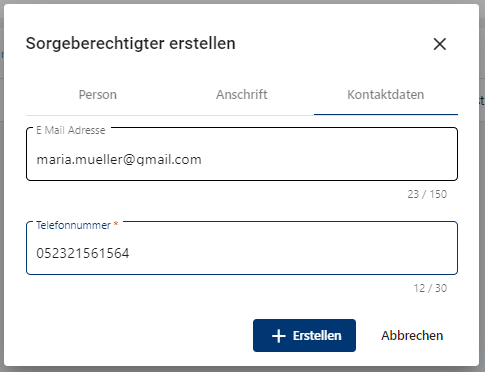
\includegraphics{sorgeberechtigter-kontakt}
    \end{adjustbox}
\end{figure}

\subsection{notfallkontakt-daten}
\begin{figure}[H]
    \centering
    \caption{Testüberschrift}
    \begin{adjustbox}{width=0.6\linewidth, center}
        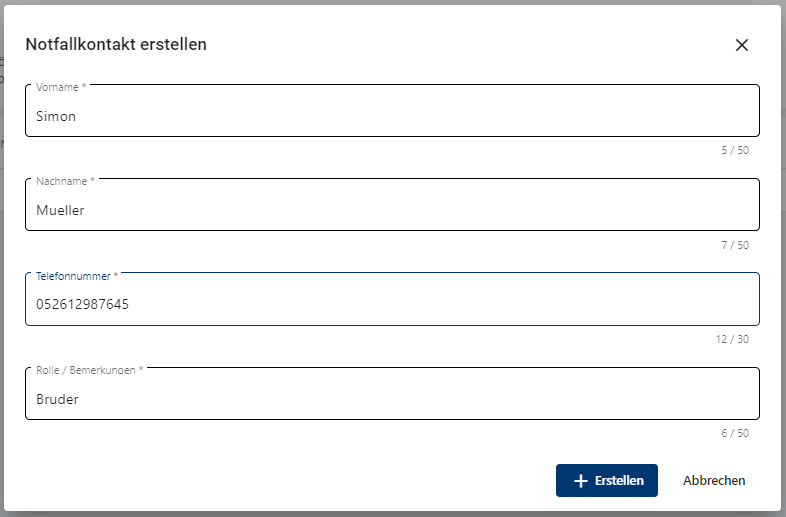
\includegraphics{notfallkontakt-daten}
    \end{adjustbox}
\end{figure}

\subsection{notfallkontakt-liste}
\begin{figure}[H]
    \centering
    \caption{Testüberschrift}
    \begin{adjustbox}{width=\linewidth, center}
        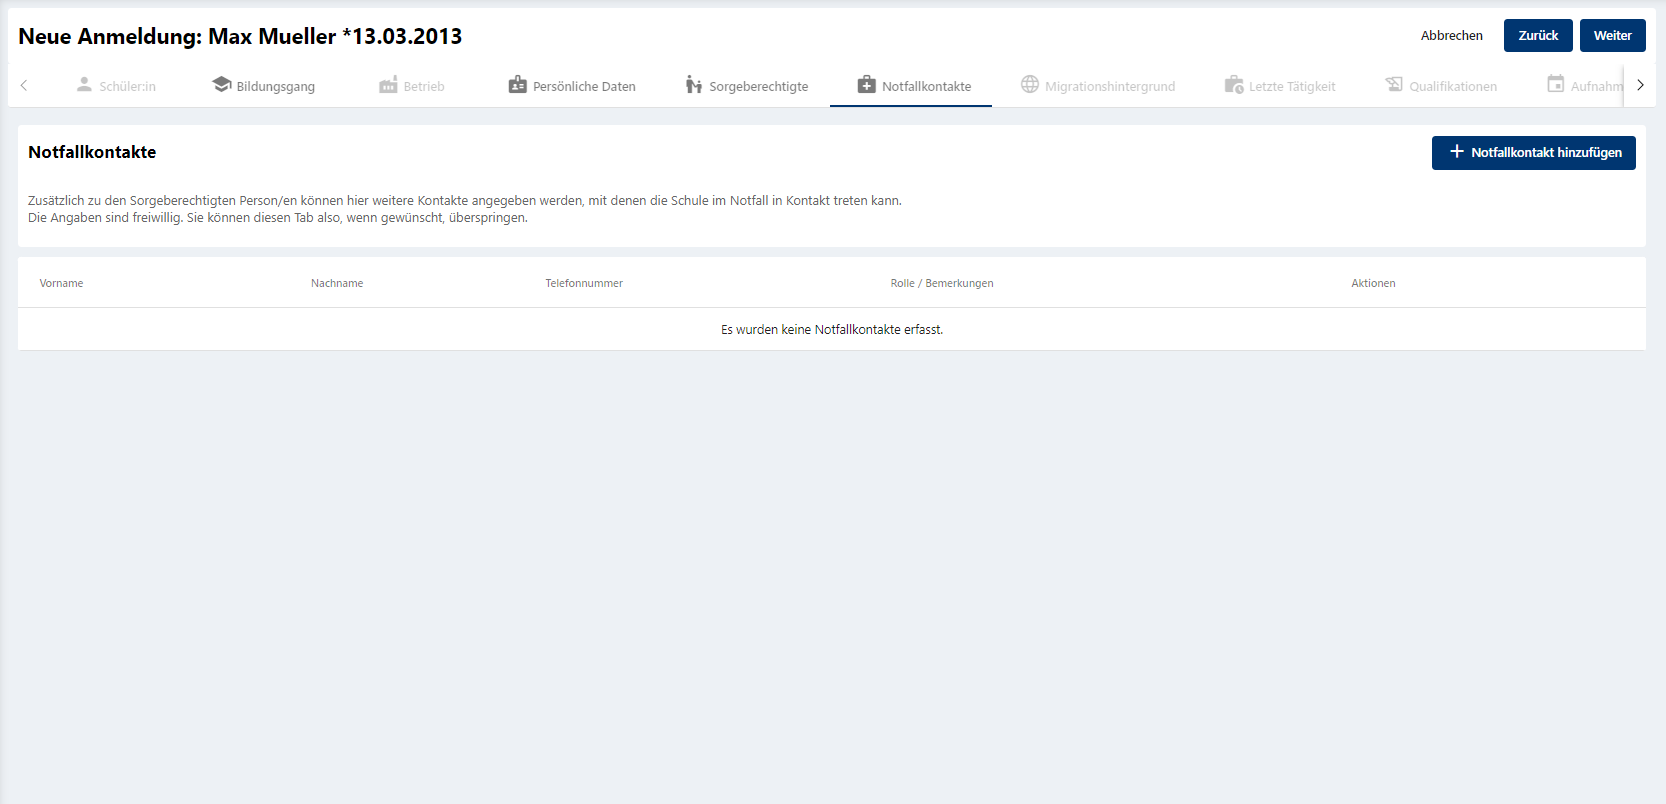
\includegraphics{notfallkontakt-liste}
    \end{adjustbox}
\end{figure}

\subsection{migrationshintergrund-liegtvor}
\begin{figure}[H]
    \centering
    \caption{Testüberschrift}
    \begin{adjustbox}{width=\linewidth, center}
        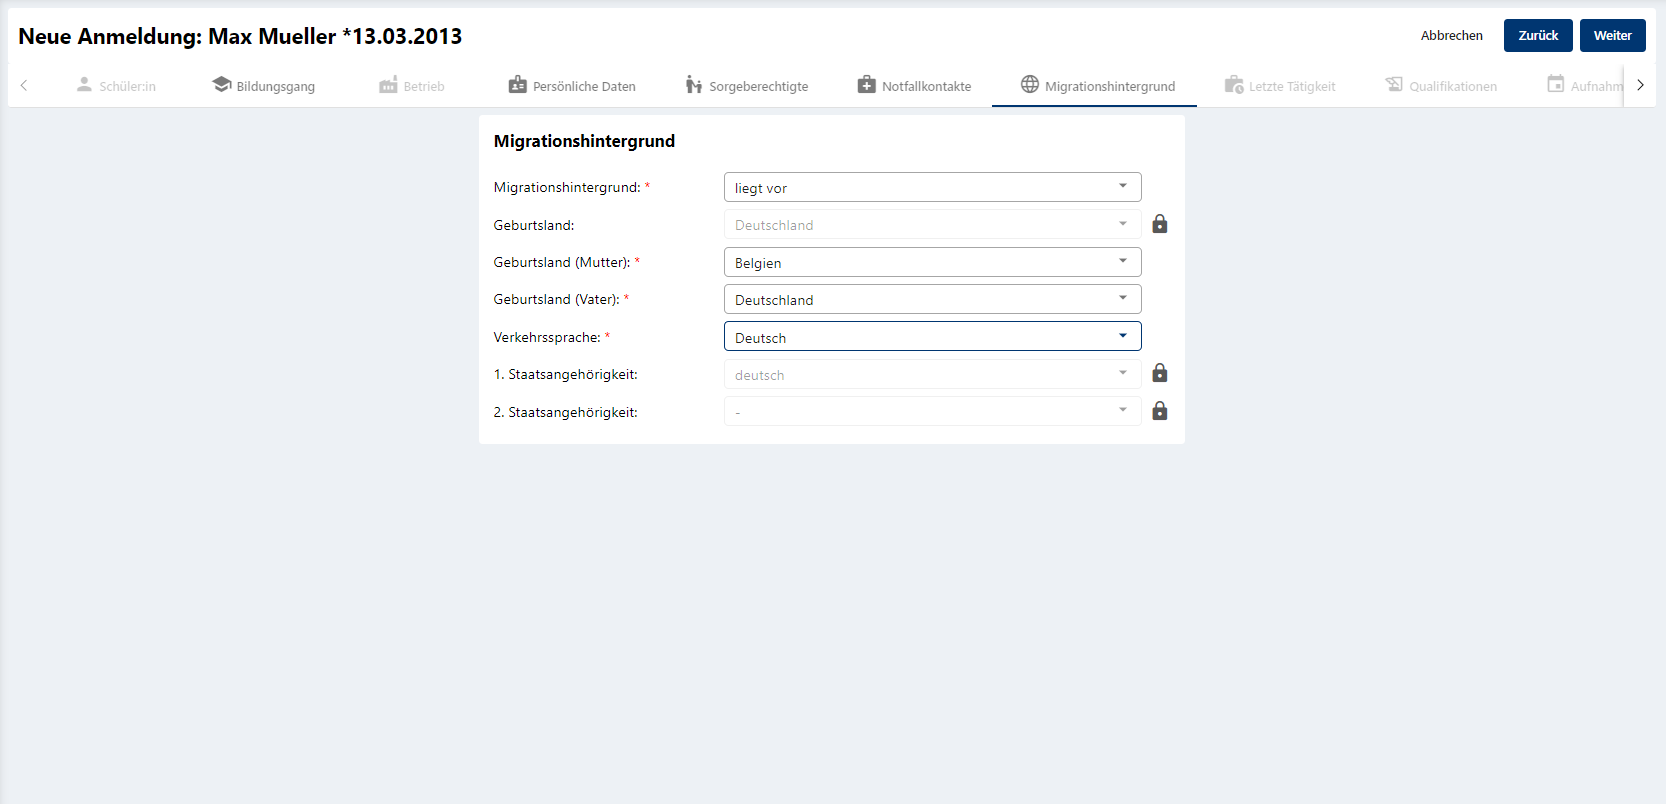
\includegraphics{migrationshintergrund-liegtvor}
    \end{adjustbox}
\end{figure}

\subsection{migrationshintergrund-liegtnichtvor}
\begin{figure}[H]
    \centering
    \caption{Testüberschrift}
    \begin{adjustbox}{width=\linewidth, center}
        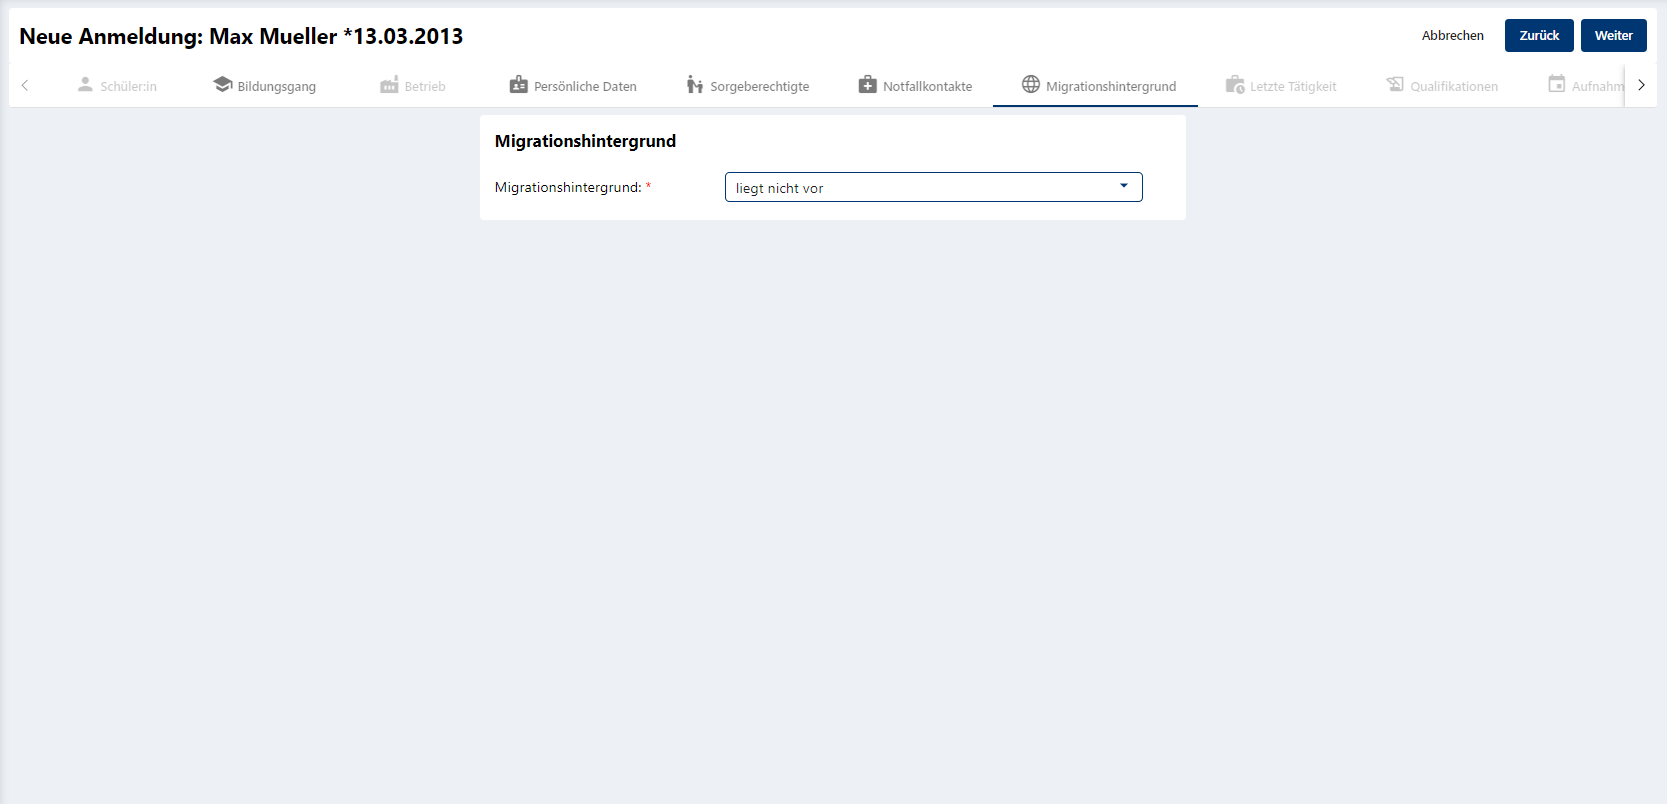
\includegraphics{migrationshintergrund-liegtnichtvor}
    \end{adjustbox}
\end{figure}

\subsection{qualifikation}
\begin{figure}[H]
    \centering
    \caption{Testüberschrift}
    \begin{adjustbox}{width=\linewidth, center}
        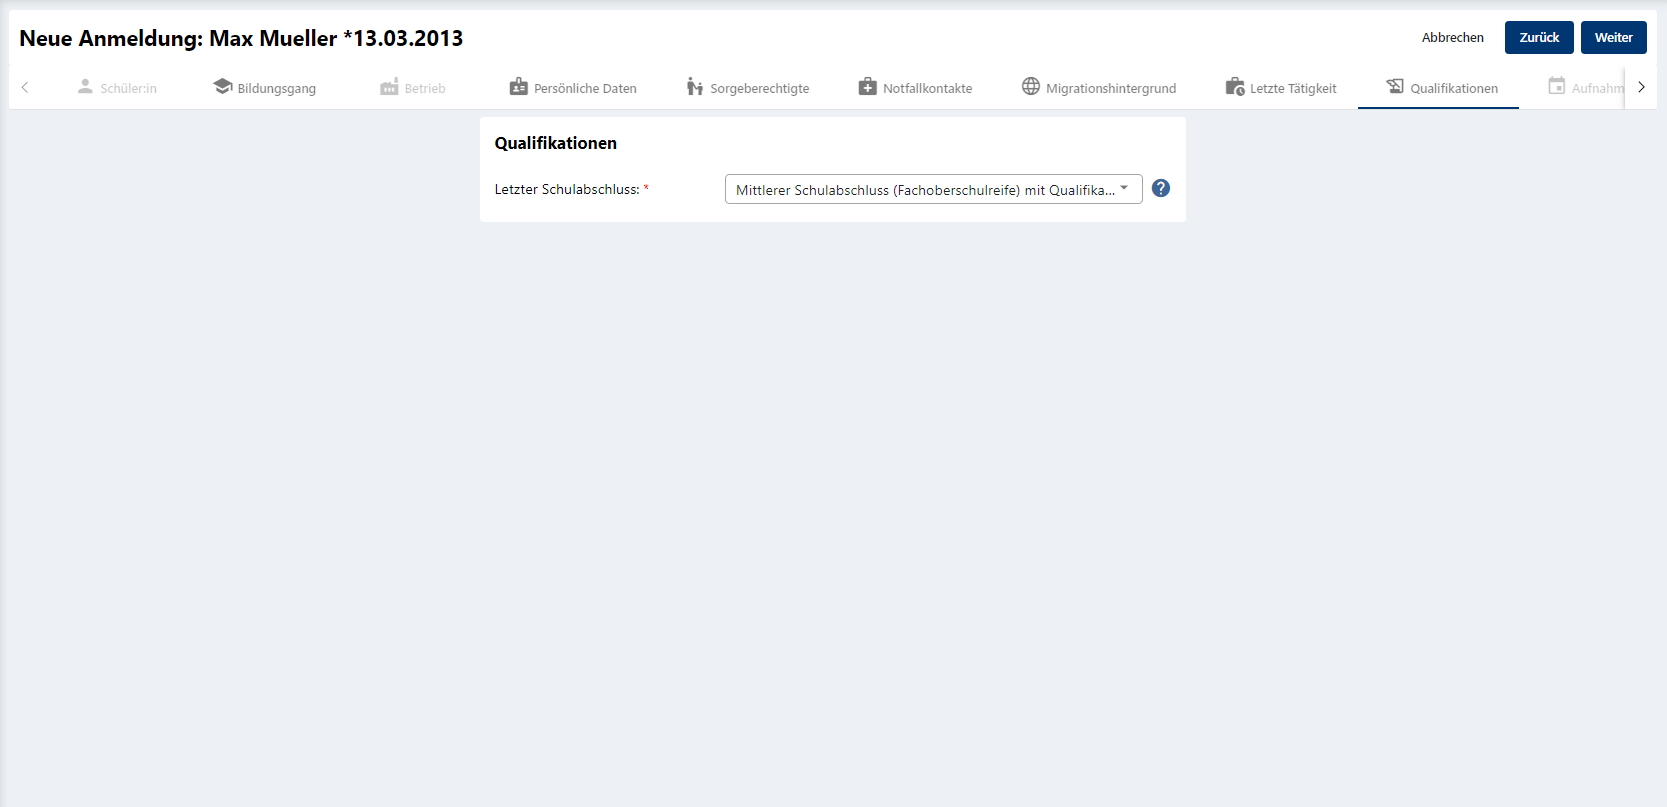
\includegraphics{qualifikation}
    \end{adjustbox}
\end{figure}

\subsection{letztetaetigkeit}
\begin{figure}[H]
    \centering
    \caption{Testüberschrift}
    \begin{adjustbox}{width=\linewidth, center}
        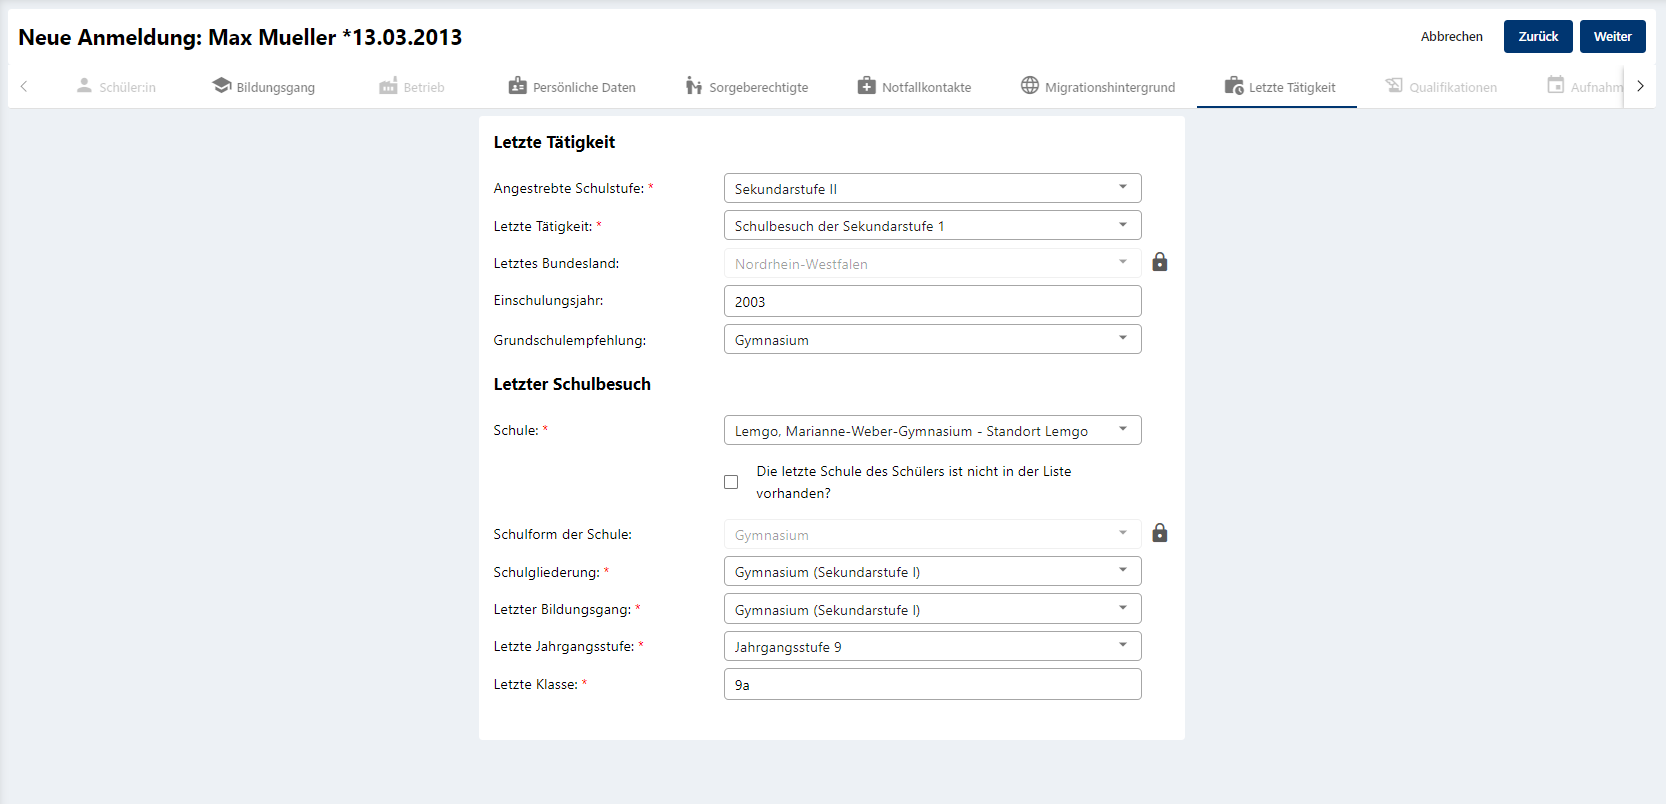
\includegraphics{letztetaetigkeit}
    \end{adjustbox}
\end{figure}

\subsection{aufnahmeberatung}
\begin{figure}[H]
    \centering
    \caption{Testüberschrift}
    \begin{adjustbox}{width=\linewidth, center}
        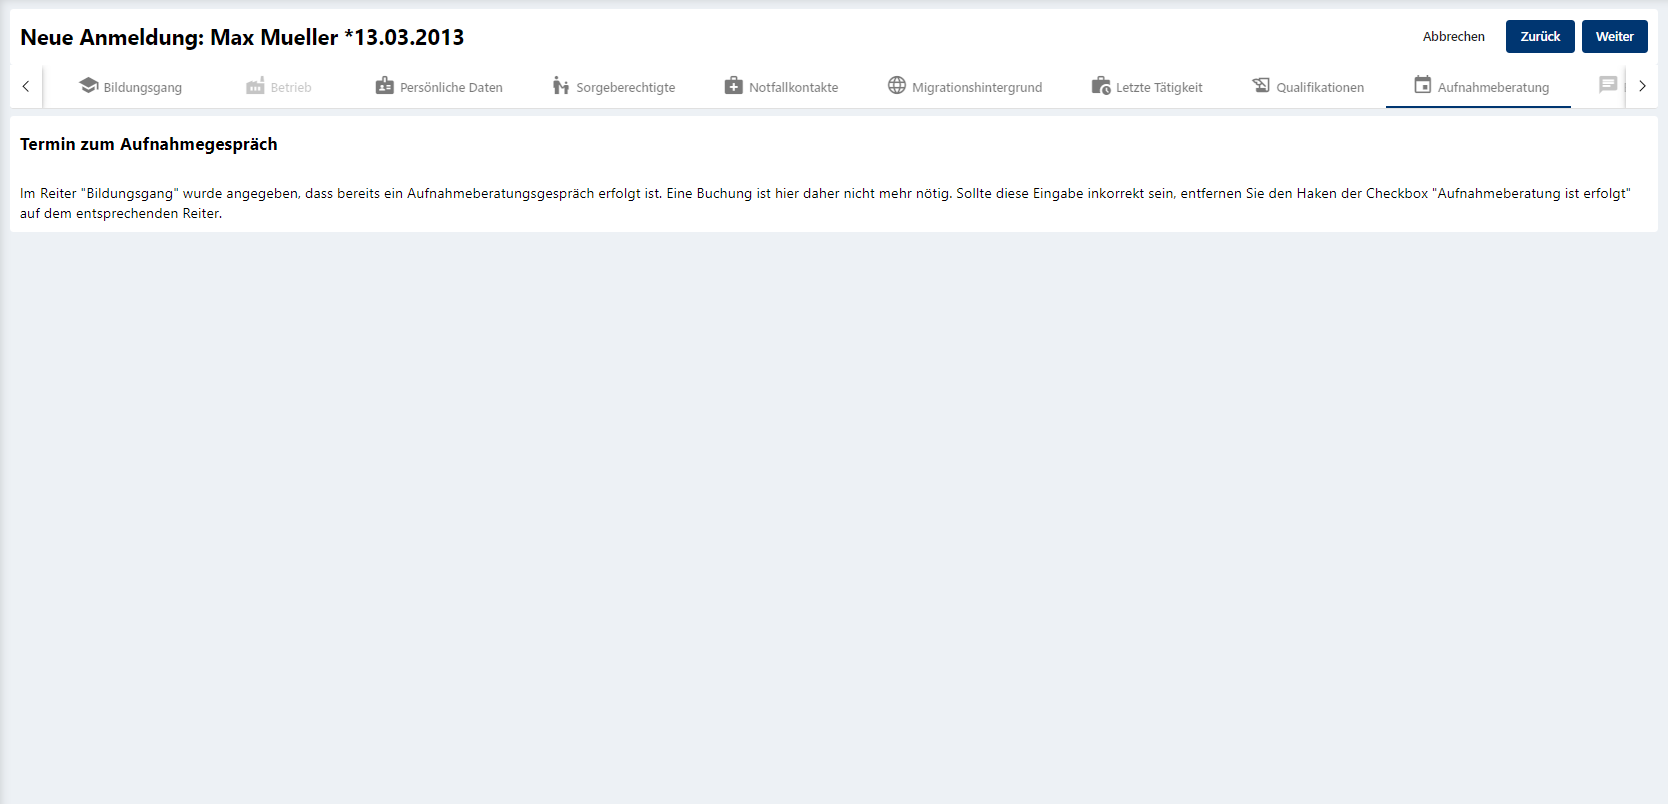
\includegraphics{aufnahmeberatung}
    \end{adjustbox}
\end{figure}

\subsection{bemerkungen}
\begin{figure}[H]
    \centering
    \caption{Testüberschrift}
    \begin{adjustbox}{width=\linewidth, center}
        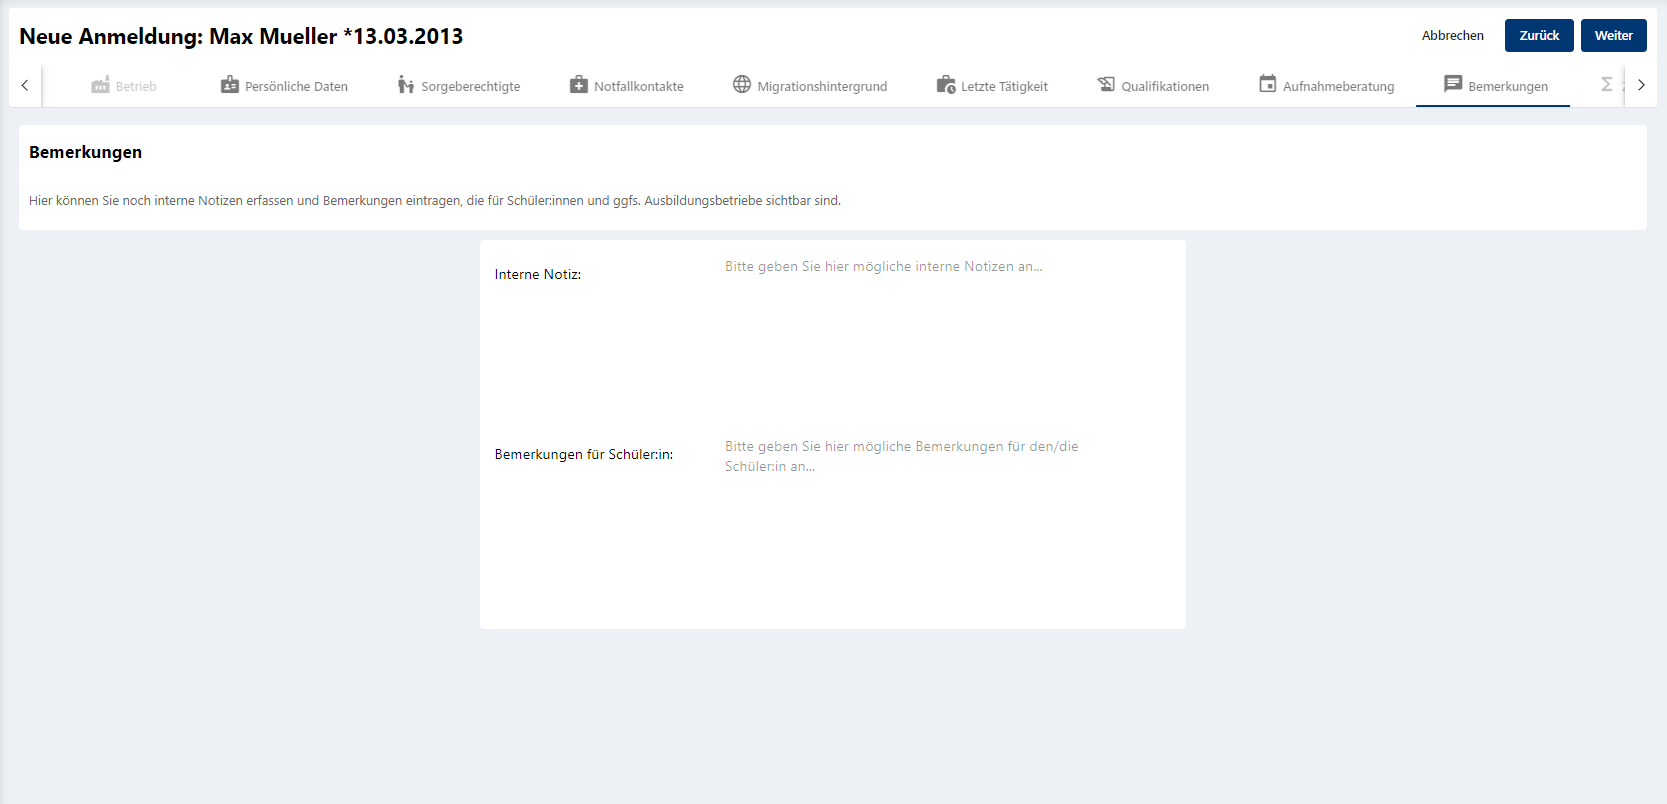
\includegraphics{bemerkungen}
    \end{adjustbox}
\end{figure}

\subsection{zusammenfassung}
\begin{figure}[H]
    \centering
    \caption{Testüberschrift}
    \begin{adjustbox}{width=\linewidth, center}
        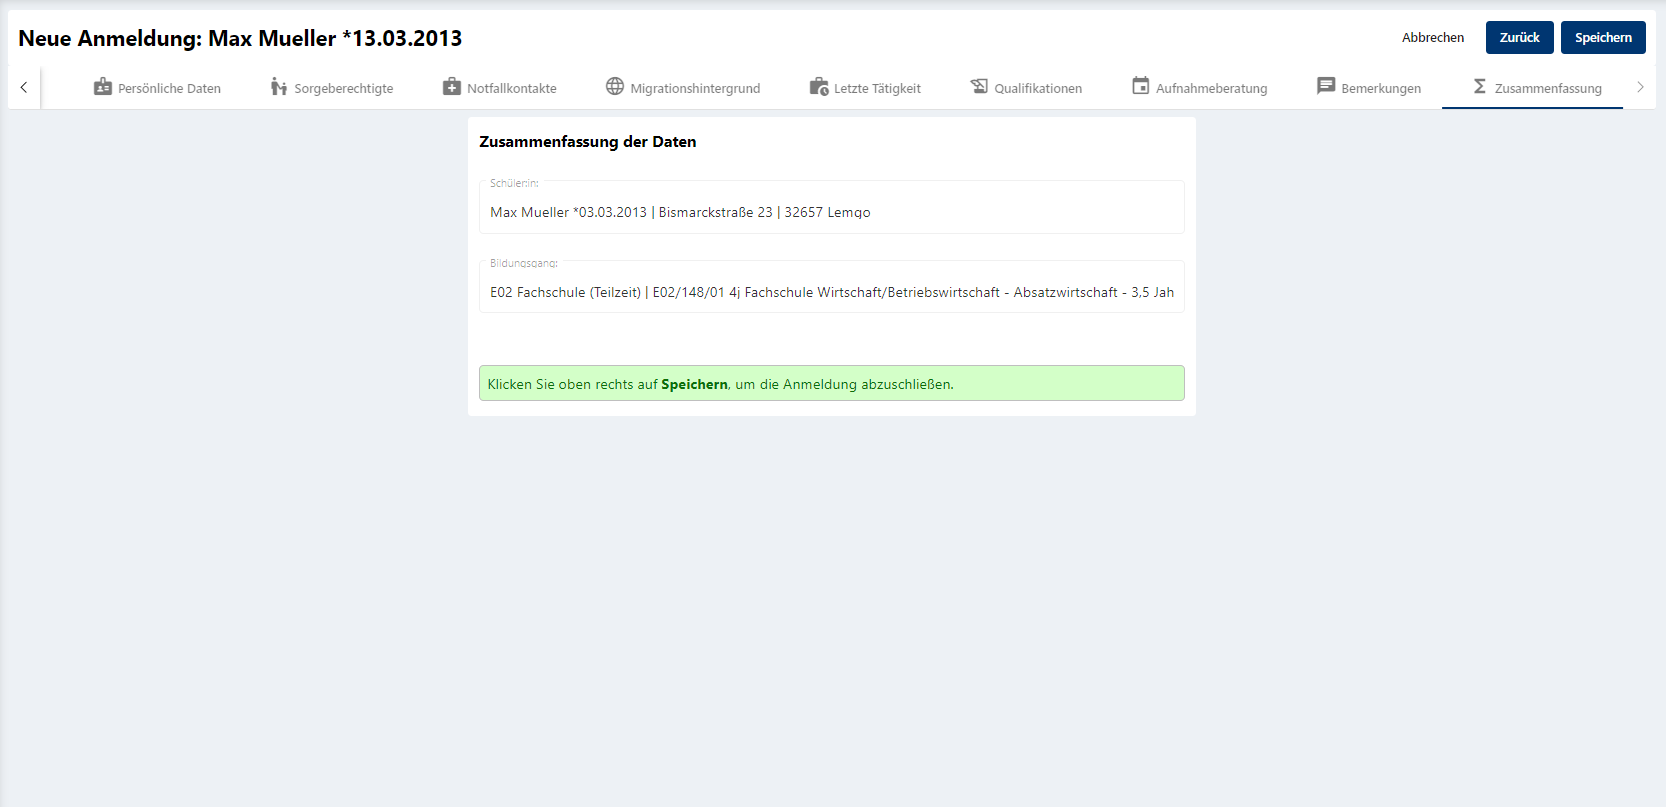
\includegraphics{zusammenfassung}
    \end{adjustbox}
\end{figure}

\subsection{bestaetigung}
\begin{figure}[H]
    \centering
    \caption{Testüberschrift}
    \begin{adjustbox}{width=\linewidth, center}
        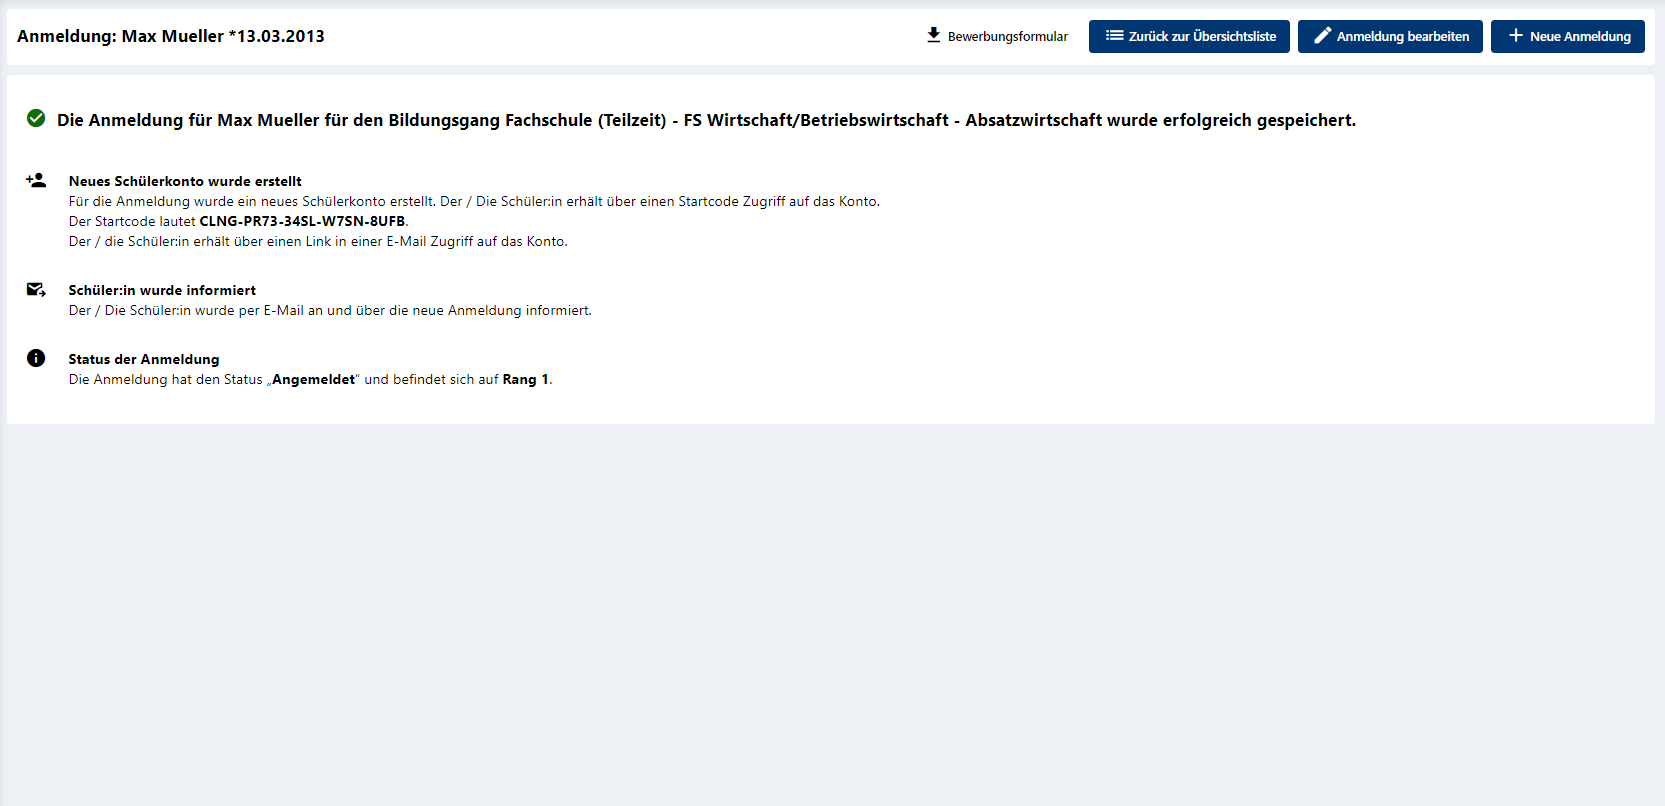
\includegraphics{bestaetigung}
    \end{adjustbox}
\end{figure}

\subsection{update-bewerbung}
\begin{figure}[H]
    \centering
    \caption{Testüberschrift}
    \begin{adjustbox}{width=\linewidth, center}
        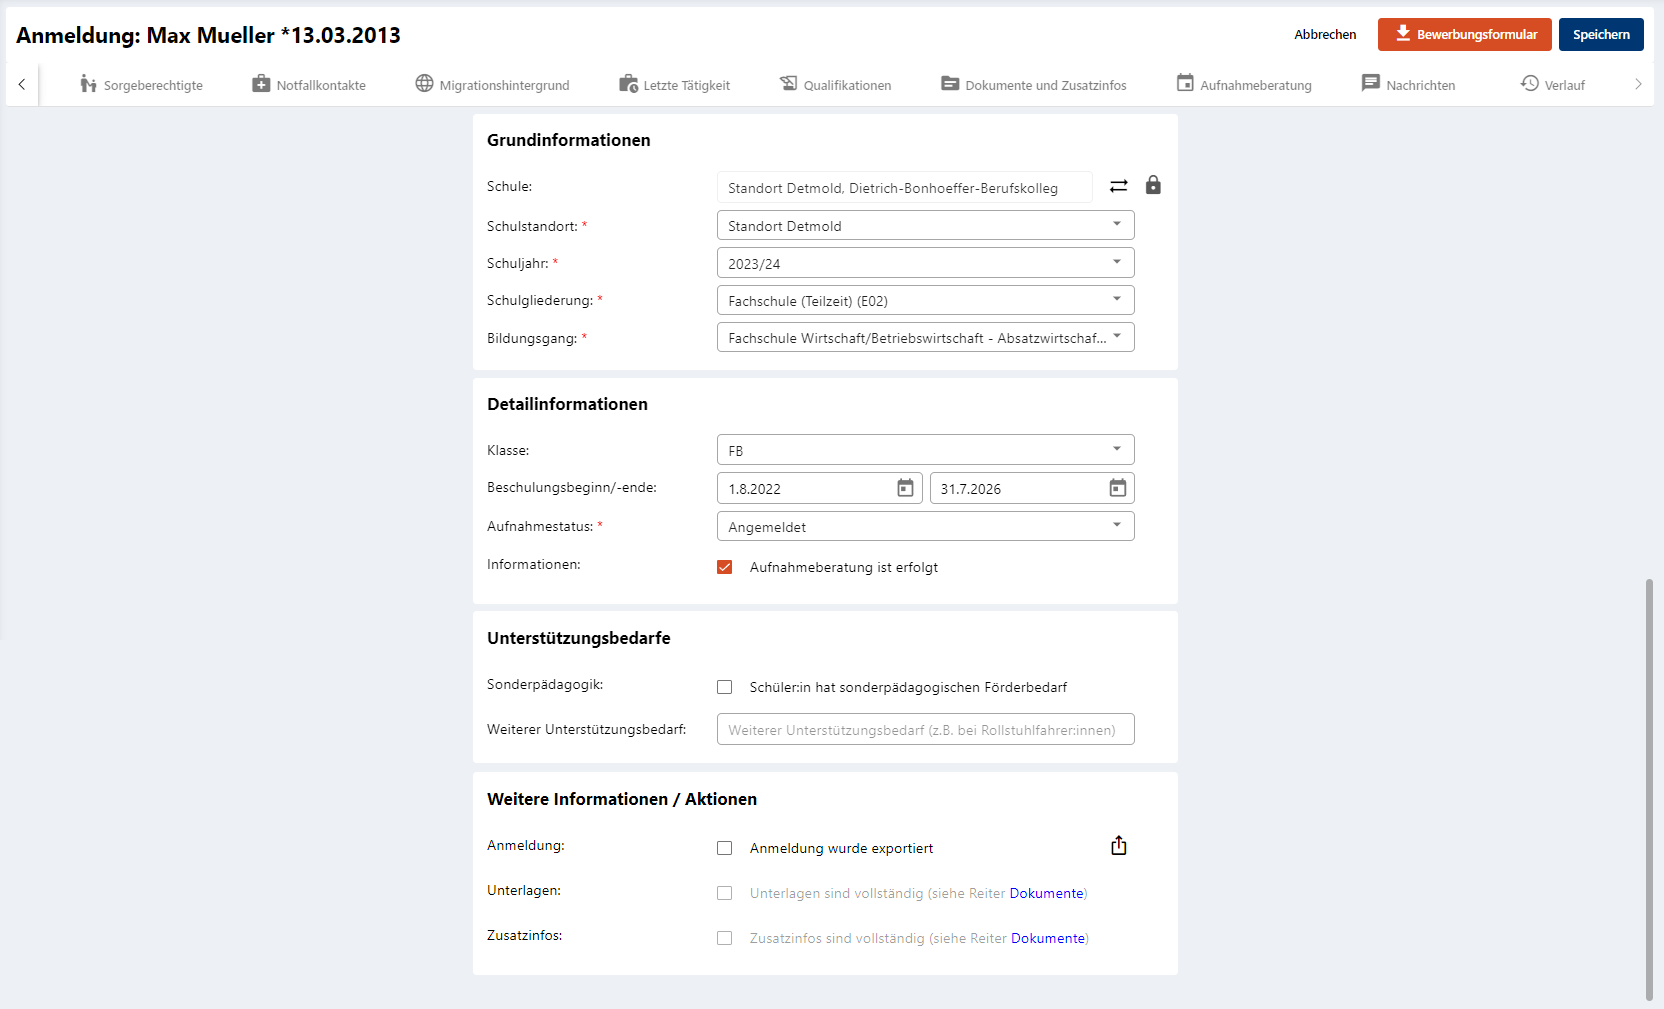
\includegraphics{update-bewerbung}
    \end{adjustbox}
\end{figure}

\end{landscape}


% Bibliographie
\printbibliography

\end{document}
